\documentclass[12pt,a4paper,twoside]{book}
\usepackage{graphicx}
\usepackage{setspace}	%double spacing for text, single for captions, footnotes, etc.
%\usepackage{hypernat} 	%substitut de cite que permet fer hyperlinks
\usepackage{natbib}		% substituye a 'hypernat' que funciona en Windows.
\usepackage[spanish]{babel}
\usepackage[utf8]{inputenc}
\usepackage{color}
\usepackage{hhline} 		% extended styles for tables
\usepackage{multirow}
\usepackage{subfigure}
\usepackage{acronym}
\usepackage{hyperref}
\usepackage{amsmath,amsmath,amssymb} 
\usepackage{fancyhdr}
\usepackage{epsfig, amsmath}
\usepackage{algorithm}
\usepackage{algorithmic}
\usepackage{enumitem}

% general settings
\hypersetup{
	linktocpage=true,
	colorlinks=true,
	linkcolor=blue,
	citecolor=blue,
}
\definecolor{Hgray}{gray}{0.6}

\newenvironment{definition}[1][Definition]{\begin{trivlist}
\item[\hskip \labelsep {\bfseries #1}]}{\end{trivlist}}

\setlength{\topmargin}{0cm}
\setlength{\textheight}{23cm}
\setlength{\textwidth}{17cm}
\setlength{\oddsidemargin}{0cm}
\setlength{\evensidemargin}{0cm}
\setlength{\headheight}{1cm}

% indica que las 'sub-sub-sections' sean numeradas y aparezcan en el indice
\setcounter{secnumdepth}{3}
\setcounter{tocdepth}{2}

% settings for code
\renewcommand{\algorithmicrequire}{\textbf{Entrada: }}
\renewcommand{\algorithmicensure}{\textbf{Salida: }}

\setlist[itemize]{noitemsep}

%%%%%%%%%%%%
% DOCUMENT %
%%%%%%%%%%%%
\begin{document}

% portada
\newpage
\thispagestyle{empty}

\baselineskip 2em

%\vspace*{1cm}

\centerline{
\includegraphics[width=0.6\textwidth]{images/UOC-logo}}
\begin{center}
\textsc{Universitat Oberta de Catalunya (UOC) \\
 Máster Universitario en Ciencia de Datos (\textit{Data Science})\\}

%\centerline {\pic{UOC}{4cm}}

\vspace*{1.5cm}

\textsc{\Large TRABAJO FINAL DE MÁSTER}

\vspace*{0.5cm}

\textsc{\large Área: Informática, Multimedia y Telecomunicación}


%\textbf{\Huge VirtualTechLab Model: }

\vspace*{2.0cm}

\textbf{\Large Predicción de Panel Attrition con Machine Learning: El caso de la Encuesta Financiera de las Familias}

\textbf{\large }

\vspace{2.5cm}
\baselineskip 1em

\baselineskip 2em
-----------------------------------------------------------------------------\\
Autor:      Carlos Luis Gento de Celis\\
Tutor:      Jordi Escayola Mansilla\\
Profesor:   Ismael Benito Altamirano\\
-----------------------------------------------------------------------------\\
\vspace*{1.5cm}
Madrid, \today

\end{center}

\newpage
\pagestyle{empty}
\hfill

\newpage
% abstract
\pagenumbering{roman} 
\setcounter{page}{1} 
\pagestyle{plain}

%%%%%%%%%%%%%%%%
%%% CREDITOS %%%
%%%%%%%%%%%%%%%%
\chapter*{Créditos/Copyright}

\vspace{1cm}

\begin{figure}[ht]
    \centering
	
\includegraphics[scale=1]{images/license.png}
\end{figure}

Esta obra está sujeta a una licencia de Reconocimiento -  NoComercial - SinObraDerivada

\href{https://creativecommons.org/licenses/by-nc-nd/3.0/es/}{3.0 España de CreativeCommons}.

%%%%%%%%%%%%%
%%% FICHA %%%
%%%%%%%%%%%%%
\chapter*{FICHA DEL TRABAJO FINAL}

\begin{table}[ht]
	\centering{}
	\renewcommand{\arraystretch}{2}
	\begin{tabular}{r | p{10cm}}
		\hline
		Título del trabajo: & Predecir panel attrition con Machine Learning: Un análisis con la Encuesta Financiera de las Familias\\
		\hline
        Nombre del autor: & Carlos Luis Gento de Celis\\
		\hline
        Nombre del colaborador/a docente: & Jordi Escayola Mansilla\\
		\hline
        Nombre del PRA: & Antonio Lozano Bagén\\
		\hline
        Fecha de entrega (mm/aaaa): & 10/2023\\
		\hline
        Titulación o programa: & Máster Universitario en Ciencia de Datos\\
		\hline
        Área del Trabajo Final: & Informática, Multimedia y Telecomunicación\\
		\hline
        Idioma del trabajo: & Español\\
		\hline
        Palabras clave & predictive models, machine learning, panel attrition\\
		\hline
	\end{tabular}
\end{table}

%%%%%%%%%%%%%%%%
%%% RESUMEN  %%%
%%%%%%%%%%%%%%%%

\chapter*{Resumen}
\addcontentsline{toc}{chapter}{Resumen}

\onehalfspacing

La Encuesta Financiera de las Familias (EFF) es una encuesta bienal cuyo objetivo es recoger información sobre la situación económico-financiera de los hogares que residen en España, y su evolución a lo largo del tiempo. Para ello, los hogares seleccionados pueden participar en hasta cuatro olas consecutivas de la encuesta. Sin embargo, hay hogares que abandonan el estudio antes de tiempo. Aunque estos abandonos no interrumpan el estudio, sí podrían afectar a sus resultados si el número de abandonos es demasiado grande, o si se concentra en colectivos específicos de la población. Es importante analizar las causas de estos abandonos y desarrollar herramientas que puedan evitarlos.

Este documento, en primer lugar, analiza las características de los hogares que participaron en la Encuesta Financiera de las Familias (EFF) en sus ediciones de 2017 y 2020, y si participaron en las olas de 2020 y de 2022. A continuación, plantea una serie modelos de predicción basados en métodos de Machine Learning y evalúa su capacidad para predecir si un hogar abandonará la EFF en 2020 o en 2022. Finalmente, interpreta los resultados el modelo que mejor ha funcionado.

\vspace{1.5cm}

\textbf{Palabras clave}: predictive models, panel attrition, machine learning, household surveys

\chapter*{Abstract}
\addcontentsline{toc}{chapter}{Abstract}

\onehalfspacing

The Spanish Survey of Household Finances (EFF) is a biennial survey whose goal is to collect information about the economical and financial situation of households in Spain, and its evolution through time. To do so, selected households may take part in up to four consecutive waves of this survey. However, some households cease their participation prematurely. Although withdrawals do not interrupt the research study, they might affect its results if the number of withdrawals is too high, or if it is more likely to happen for certain groups of people. It is important to analyse the causes of this phenomenon and develop tools to prevent it.

Firstly, this paper analyses the characteristics of households that responded to the EFF in its editions of 2017 and 2020, and their participation during the 2020 or 2022 waves. Next, a series of predictive models based on machine learning methods are considered and evaluated for the exercise of predicting panel attrition in the EFF. Finally, it interprets the results of the most successful model.

\vspace{1.5cm}

\textbf{Key words}: predictive models, panel attrition, machine learning, longitudinal surveys, household surveys
\newpage

\pagestyle{fancy}
\renewcommand{\chaptermark}[1]{ \markboth{#1}{}}
\renewcommand{\sectionmark}[1]{\markright{ \thesection.\ #1}}
\lhead[\fancyplain{}{\bfseries\thepage}]{\fancyplain{}{\bfseries\rightmark}}
\rhead[\fancyplain{}{\bfseries\leftmark}]{\fancyplain{}{\bfseries\thepage}}
\cfoot{}

% indice
\cleardoublepage
\phantomsection
\addcontentsline{toc}{chapter}{Índice}
\tableofcontents

\thispagestyle{empty}

\pagenumbering{arabic}

\pagestyle{fancy}
\renewcommand{\chaptermark}[1]{ \markboth{#1}{}}
\renewcommand{\sectionmark}[1]{\markright{ \thesection.\ #1}}
\lhead[\fancyplain{}{\bfseries\thepage}]{\fancyplain{}{\bfseries\rightmark}}
\rhead[\fancyplain{}{\bfseries\leftmark}]{\fancyplain{}{\bfseries\thepage}}
\cfoot{}

\onehalfspacing

% capitulos del documento
\chapter{Introducción}
\label{chapter:introduccion}

Los estudios longitudinales son proyectos de investigación en los que se hace un seguimiento a un grupo de unidades muestrales (personas, hogares...) a lo largo de un período de tiempo. En el ámbito de las ciencias sociales, la recolección de datos de muchos de estos estudios se realiza mediante el uso de encuestas, de tal manera que las mismas personas responden a las preguntas del mismo cuestionario de manera repetida durante un tiempo, que pueden ser semanas, meses o incluso años. Esto da lugar a las llamadas encuestas longitudinales o encuestas panel. La dimensión temporal de estas encuestas las convierten en una herramienta muy útil para poder analizar relaciones causales, ya que permiten observar cambios en opiniones, comportamientos o estados de los mismos panelistas a lo largo del tiempo. Sin embargo, la calidad de esos análisis depende de la cooperación exitosa y continuada de dichos panelistas durante las sucesivas ediciones u olas de la encuesta. El abandono prematuro y acumulado en el tiempo de participantes en un panel se conoce como \textbf{Panel Attrition} (\cite{watson2009identifying}).

\cite{lynn2018tackling} destaca que el Panel Attrition presenta dos principales problemas. Por un lado, si la tasa de abandonos es alta, el tamaño de la muestra se reducirá drásticamente en pocas olas, lo que provocará que la precisión de los estimadores de la encuesta sea muy baja, y además limitará o incluso imposibilitará el análisis de subgrupos dentro de la muestra. Por otro lado, si el Panel Attrition no es aleatorio y los panelistas que abandonan la encuesta son sistemáticamente diferentes a los que se mantienen, existe el riesgo de introducir un sesgo de no-respuesta en los estimadores de la encuesta.

Tradicionalmente, los métodos utilizados para mitigar los efectos del Panel Attrition se han centrado en el impacto estadístico que provoca, principalmente con el uso de métodos de imputación múltiple (\cite{rubin1987multiple}), la reponderación de pesos muestrales (\cite{groves2009survey}) e introduciendo muestras de refresco para sustituir a las unidades muestrales perdidas (\cite{hirano1998combining}). Pero en las últimas décadas ha aumentado el interés por tratarlo durante los procesos de creación y recolección de datos, lo que ha llevado a la extensión del uso de los llamados diseños adaptativos y reactivos (adaptative and responsive designs, \cite{tourangeau2017adaptive}). La idea detrás de estos diseños se fundamenta en utilizar toda la información que se genera durante la elaboración de encuestas (respuestas al cuestionario, paradata u observaciones de los entrevistadores) para diseñar implementaciones informadas cuyo objetivo sea mejorar la calidad de los datos, reducir los costes, o ambos. En este sentido, las encuestas longitudinales ofrecen una gran oportunidad para estos diseños porque contienen mucha información tanto de los trabajos de campo que se estén desarrollando, como los que se realizaron en olas anteriores. Por ejemplo, se ha utilizado información sobre intentos de contacto en olas pasadas para revisar la estrategia de incentivos para hogares a los que cuesta volver a entrevistar (\cite{mcgonagle2022effects}) o para optimizar las estrategias de contacto en las ediciones siguientes (\cite{kreuter2015note}).

Dentro de este contexto de los diseños adaptativos y reactivos, en las últimas décadas se ha desarrollado el uso algoritmos de Machine Learning en la metodología de encuestas, especialmente para predecir Panel Attrition (\cite{buskirk2018introduction}). Por ejemplo, en \cite{beste2023case} utilizan información de ediciones pasadas de una encuesta a hogares en Alemania para entrenar varios modelos basados en algoritmos de Machine Learning para identificar hogares panelistas con una baja probabilidad de volver a participar en la siguiente edición. Posteriormente, utilizan el mejor de esos modelos para predecir cuáles hogares panelistas de una nueva edición tenían menor probabilidad de colaborar de nuevo, y usan esas predicciones para crear un diseño experimental enfocado en esos hogares.

El objetivo de este Trabajo de Fin de Máster es adaptar la implementación de Machine Learning vista en \cite{beste2023case} para predecir la participación de los hogares panel al caso de estudio de la Encuesta Financiera de las Familias (EFF). La EFF es una encuesta a hogares representativa de los hogares que residen en España, y es creada por el Banco de España. La idea central del ejercicio de predicción consiste en utilizar información de hogares en olas pasadas de la EFF para predecir una variable binaria de participación o no participación en la ola siguiente. Para ello, se entrenan cuatro modelos basados en algoritmos de Machine Learning y se compara su rendimiento con un modelo de referencia utilizado tradicionalmente en análisis de Panel Attrition, que en este caso es una Regresión Logística o Logit. En este proyecto, para el entrenamiento de los modelos se utiliza información sobre hogares que han participado en las olas 4, 5, 6 y 7 de la EFF (que se corresponden con los años 2011, 2014, 2017 y 2020), y a continuación se utilizan dichos modelos para predecir la participación de los hogares panel elegibles para la ola 8 (que se corresponde con el año 2022).

Los seis capítulos restantes de este documento se organizan de la siguiente manera. En el siguiente capítulo se exponen los objetivos, la planificación del proyecto y las motivaciones personales para realizarlo. En el tercer capítulo se hace una revisión del estado del arte para este estudio, en el que se describe cuáles son las causas del Panel Attrition, cómo se están utilizado algoritmos de Machine Learning para predecirlo, y finalmente se presenta la Encuesta Financiera de las Familias (EFF). En el cuarto capítulo se describe la metodología utilizada en el análisis exploratorio de datos y en el ejercicio de entrenamiento, validación y test de los modelos de predicción de Panel Attrition. En el quinto capítulo se presentan los datos de la EFF y se realizan una descripción de las etapas de producción de la EFF, y un análisis exploratorio de los datos. En el sexto capítulo se muestran y comentan los resultados del entrenamiento y la evaluación de los modelos de predicción, y se analiza la importancia de las variables utilizadas en uno de los modelos de predicción para explicar el Panel Attrition. Finalmente, en el último capítulo se exponen las conclusiones y reflexiones sobre el proyecto y cuáles pueden ser las líneas de trabajo para el futuro.
\chapter{Objetivos del proyecto, planificación y motivación personal}
\label{chapter:objetivos}
\section{Objetivos del proyecto}

Este proyecto se contextualiza dentro del marco de la metodología de encuestas. En concreto, se centra en las encuestas longitudinales a hogares, y dentro de ese campo pone el foco en la predicción de la participación de los hogares en olas posteriores a su primera colaboración. La encuesta elegida para el proyecto es la Encuesta Financiera de las Familias (EFF), una encuesta de referencia para investigaciones sobre finanzas de los hogares.

El \textbf{objetivo principal} de este proyecto es desarrollar un modelo de predicción basado en métodos de machine learning que ayude a predecir si un hogar que ha participado en al menos una ola de la EFF volverá a hacerlo en olas posteriores.

Para poder desarrollar ese modelo, es necesario completar una serie de \textbf{objetivos secundarios}. Estos objetivos se agruparán en 5 fases:

\begin{enumerate}[noitemsep]
    \item Hacer una revisión del estado del arte sobre el Panel Attrition y las metodologías de Machine Learning aplicadas a su predicción.
    \item Recolección de datos. Preferentemente, obtener un conjunto de datos que contenga:
    \begin{enumerate}
        \item Las respuestas de los hogares al cuestionario de la EFF.
        \item Paradata sobre el proceso de creación de la encuesta.
        \item Características de los entrevistadores.
    \end{enumerate}
    \item Análisis exploratorio de los datos. Identificar patrones dentro de los datos que puedan estar relacionados con el panel attrition.
    \item Preprocesar los datos para entrenar modelos de machine learning.
    \item Modelado y evaluación de modelos de predicción basados en métodos de machine learning.
    \item Interpretación del mejor modelo y redacción de conclusiones.
\end{enumerate}

\section{Planificación del proyecto}

La planificación de este proyecto se va a dividir en 5 fases. La asignación temporal a cada una de ellas se ha realizado de acuerdo a la estructura de contenidos del Plan Docente y al calendario de la asginatura.

\begin{enumerate}[noitemsep]
    \item Fase 1: Contiene la definición del proyecto y la planificación del TFM. Abarca las dos primeras semanas del proyecto, del 27 de septiembre al 10 de octubre.
    \item Fase 2: Contiene las tareas de la revisión de la literatura y la caracterización del panel attrition de la EFF. Abarcará desde el 11 de octubre al 23 de octubre.
    \item Fase 3: Contiene las tareas de recolección de datos, análisis exploratorio de dichos datos, preprocesamiento para entrenar los modelos de machine learning, modelado y evaluación de los modelos de predicción, y la interpretación de los modelos y la redacción de conclusiones. Esta fase es la más duradera y abarcará desde el 17 de octubre al 19 de diciembre.
    \item Fase 4: En esta fase se procederá a la redacción de la memoria del TFM y la preparación de una presentación audiovisual sobre el proyecto. Abarcará desde el 20 de diciembre al 18 de enero.
    \item Fase 5: En esta fase final se procederá a la defensa del TFM. Esa etapa abarcará desde el 22 de enero hasta el 4 de febrero.
\end{enumerate}

 En la figura \ref{fig:gantt} puede observarse la distribución temporal y el tiempo dedicado a cada tarea en un diagrama de Gantt.


\begin{figure}
	\centering
	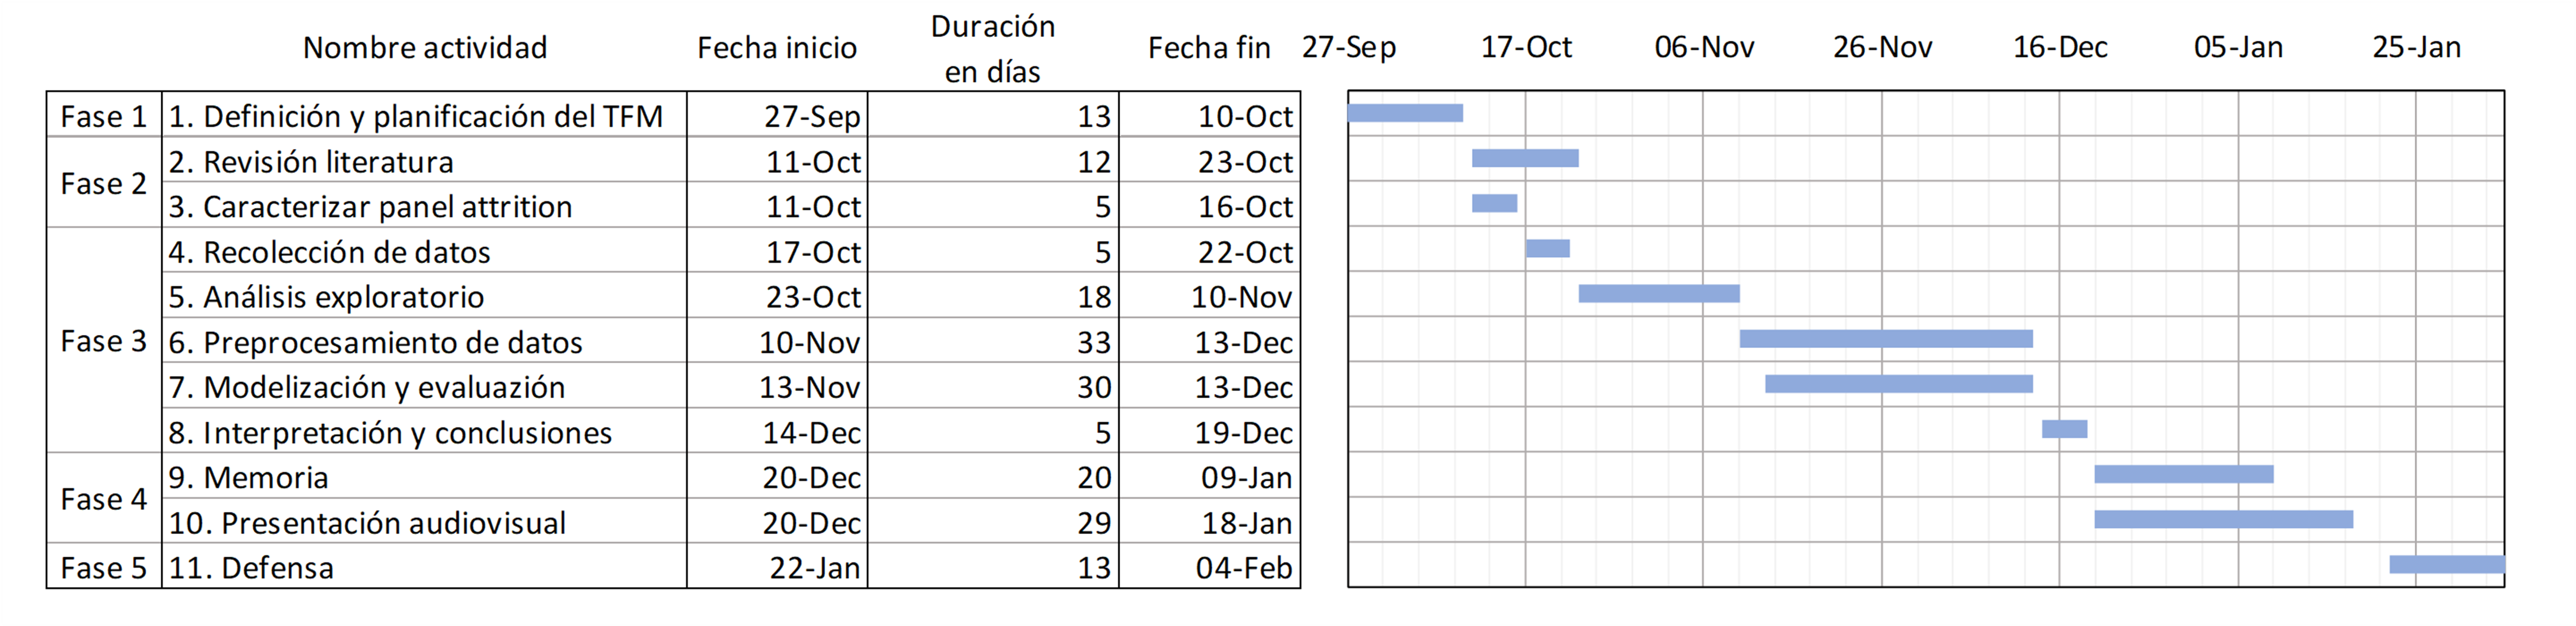
\includegraphics[width=1\textwidth]{figs/Gantt_diagram.png}
	\caption{Planificación de las actividades del TFM}
	\label{fig:gantt}
\end{figure}

\section{Motivación personal}

Trabajo para el Banco de España, y formo parte del equipo que elabora la Encuesta Financiera de las Familias (EFF) desde principios de 2015. He participado en la elaboración de sus cuatro últimas ediciones (EFF2014, EFF2017, EFF2020 y EFF2022) y con los años ha crecido mi interés por la metodología de encuestas y el potencial que tienen para recoger información sobre fenónemos que de otra manera serían difíciles de captar. La EFF es una fuente de información de referencia en el campo de las finanzas de los hogares y eso hace más importante realizar trabajos y esfuerzos para garantizar e incluso mejorar la calidad de sus datos. En ese sentido, la gran cantidad de paradatos que se generan durante cada ola ofrecen muchas oportunidades para aprender sobre todo el proceso y encontrar maneras de mejorarlo.

Por otro lado, en los últimos años ha aumentado cantidad de datos que se generan durante la encuesta y también su variedad, tomando espacecial relevancia los audios de las entrevistas y los comentarios de texto escritos por los entrevistadores, que se han convertido en herramientas fundamentales de los procesos de revisión de calidad de los datos. Los métodos y las herramientas desarrolladas en el campo de la ciencia de datos abren un mundo de posibilidades para poder analizar y explotar toda esa información.

Finalmente, sobre el Panel Attrition, considero que la etapa más importante de la elaboración de la EFF es el trabajo de campo. En ella se contacta a los hogares, se les convence para participar en la encuesta y se realizan las entrevistas. Marca el devenir las siguientes etapas, y también el nivel de calidad de los datos. Por esa razón, es importante conseguir la colaboración de los hogares. Especialmente la de los hogares panel, ya que representan una proporción importante de la muestra, y no convercerles puede llegar a ser muy costoso. Y es un área que en la EFF no se ha podido explorar hasta. Es una gran oportunidad para aprender.
\chapter{Estado del Arte}
\label{chapter:attrition}
\section{Causas del Panel Attrition}
\label{section:causes_attrition}

Tal y como hemos mencionado en la introducción, los diseños adaptativos y reactivos buscan implementar intervenciones en los procesos de creación de datos de encuestas. Para poder implementarlas para reducir el abandono de panelistas, es importante conocer qué provoca el abandono de los hogares panelistas. Conceptualmente, las causas del Panel Attrition pueden clasificarse en tres categorías secuenciales (\cite{lepkowski2002nonresponse}): no-localización, no-contacto y no-cooperación.

La no-localización se refiere a no localizar exitosamente a un encuestado durante una ola posterior. Generalmente, esto se debe a cambios en la información de contacto (dirección de residencia, número teléfono, correo electrónico...) obtenida del participante durante la ola anterior (\cite{couper2009keeping}). Algunos factores que pueden contribuir al éxito o fracaso en la localización son el método de recolección de datos, la propensión a los cambios de localización de los encuestados entre diferentes olas, el tiempo transcurrido entre olas e incluso el presupuesto (\cite{lynn2009methods}). Por ejemplo, las encuestas con entrevistas cara a cara utilizan métodos de rastreo y búsqueda que suelen ofrecer altos índices de localización y cooperación (\cite{de2005mix}, \cite{couper2009keeping}), pero también requieren esfuerzos adicionales para localizar a los participantes panel que se hayan mudado, como por ejemplo reembolsar a los entrevistadores los gastos derivados del proceso de búsqueda.

La segunda causa es el no-contacto. Tras localizar exitosamente al encuestado, es necesario establecer un contacto. Para que sea exitoso, es necesario que el intento de contacto por parte de los encuestadores coincida temporalmente con la disponibilidad del panelista. Esto depende completamente del método de recolección de los datos. Por ejemplo, en una entrevista personal, el panelista debe estar en su residencia justo en el mismo momento en el que la persona que quiere entrevistarle hace la visita al hogar. Algo parecido sucede con las entrevistas telefónicas, ya que el panelista debe tener su teléfono accesible cuando se realiza la llamada para intentar el contacto. Tradicionalmente, dos estrategias de contacto que han presentado buenos resultados han sido utilizar un número de intentos de contacto alto y diversificado en horarios (mañana, tarde, fines de semana...), y establecer períodos para realizar entrevistas lo suficientemente largos (\cite{nicoletti2005survey}, \cite{watson2009identifying}).

Finalmente, tras establecer el contacto, es necesario convencer al panelista para que vuelva a participar otra vez en la encuesta. La falta de cooperación es una preocupación común en todo tipo de encuestas, y suelen destacar factores como las características socio-demográficas de los encuestados o la temática de la encuesta (\cite{groves1992understanding}). En el caso particular de las encuestas longitudinales, los encuestados además poseen una experiencia previa por haber participado en ediciones pasadas. Esto hace que sea relativamente probable que vuelvan a hacerlo, en parte por ser consistentes con su comportamiento de conformidad mostrado anteriormente (\cite{groves1992understanding}), pero también puede potenciar el efecto negativo de factores como la duración de la entrevista, la carga cognitiva que supone pensar algunas respuestas o la fatiga por haber participado en varias ediciones anteriores (\cite{laurie1999strategies}, \cite{watson2009identifying}, \cite{lynn2018tackling}).

En el siguiente apartado se comenta cómo la disponibilidad de información sobre todas estas causas puede ser aprovechada por los algoritmos de Machine Learning para crear modelos que ayuden a predecir Panel Attrition, y posibilitar la implementación de diseños adaptativos y reactivos con el objetivo de reducir el abandono de hogares panelistas en encuestas longitudinales.

\section{Predicción de Panel Attrition con Machine Learning}

Los modelos utilizados en metodología de encuestas pueden clasificarse en dos categorías según sus objetivos: modelos para explicar, y modelos para predecir. Los modelos explicativos utilizan toda la información disponible para explorar las relaciones entre diferentes variables observadas, identificar causalidad entre ellas y realizar ejercicios de inferencia y contrastes de hipótesis. Los modelos predictivos, en cambio, buscan predecir o clasificar con precisión el valor de ciertas variables para escenarios que todavía no han ocurrido. Por construcción, sólo utilizan la información disponible antes de que ocurra el suceso a predecir. Aunque los modelos basados en algoritmos de Machine Learning pueden ser utilizados para ambas tareas, son particularmente interesantes para realizar tareas de predicción. En \cite{buskirk2018introduction} destacan particularmente la flexibilidad de los modelos de Machine Learning con respecto a otros modelos tradicionales utilizados en la metodología de encuestas, como la regresión logística o los mínimos cuadrados ordinarios (OLS). Para muchos algoritmos de Machine Learning no es necesario hacer supuestos sobre las distribuciones de las variables, hacer una especificación explícita de las relaciones entre variables antes de estimar los modelos, y además soportan el uso de un gran número de variables. Esto les permite detectar patrones y relaciones complejas entre variables y los convierte en una herramienta muy útil para realizar tareas de predicción.

En el contexto de la predicción del Panel Attrition, muchos estudios comparan el rendimiento de modelos de Machine Learning con el de modelos que se han utilizado tradicionalmente para analizar Panel Attrition, generalmente una regresión logística o Logit de efectos principales, es decir, sin considerar interacciones entre variables ni relaciones no linales. En \cite{kern2019tree} y \cite{kern2021predicting} utilizan datos de dos paneles de hogares en alemania para comparar el rendimiento de un Logit con varios modelos basados en árboles de decisión. Los resultados son prometedores ya que todos los modelos basados en árboles mostraron mejores rendimientos que el Logit, y además destacan por su facilidad para ser interpretados.

Otro ejemplo prometedor, y que además sirve para implementar un diseño adaptativo, puede verse en \cite{beste2023case}. Este estudio se divide en dos partes. En primer lugar, se utiliza información de ediciones pasadas de una encuesta a hogares en Alemania para comparar, de nuevo, el rendimiento de un Logit con un algoritmo k-nearest neighbours (kNN), un árbol de clasificación (CART), un Random Forest (RF) y un Gradient Boosting Machine (GBM). El modelo que ofreció mejores resultados fue el Random Forest. Y en la segunda parte, utilizaron ese modelo de Random Forest para identificar hogares panelistas con una baja propensión a participar en la edición siguiente de la encuesta. Esa información les sirvió para crear un diseño experimental en el cual se asignaba un incentivo monetario adicional a la mitad de ésos hogares. Los resultados del experimento mostraron incrementos en las tasas de respuesta de los hogares tratados, y animaron a sus responsables a seguir utilizando este diseño adaptativo en futuras ediciones.

Aunque sin duda estos resultados son prometedores, es importante recalcar que deben contextualizar y valorar para cada caso particular de análisis. Por ejemplo, en \cite{liu2020using} se utiliza un panel de individuos en Estados Unidos para predecir la participación de panelistas en la segunda edición de dicha encuesta, y se compara de nuevo el rendimiento de un Logit con los de un Random Forest (RF), un modelo de Máquinas de Soporte Vectorial (SVM) y un LASSO. Sólo el LASSO mostró una mejora con respecto al modelo de regresión logística. Otro ejemplo puede verse en \cite{jankowsky2022validation}. En este estudio se compara el rendimiento de un modelo Logit con el de un modelo GBM (Gradient Boosting Machine) en dos encuestas con diseños bastante diferentes (una encuesta es en EEUU y la otra en Alemania, una se ha realizado cada nueve años y la otra anualmente, una es telefónica y la otra es una entrevista presencial...). Para ambas encuestas apenas se observa que el GBM mejore los resultados de la regresión logística.

Como resumen, podemos decir que los algoritmos de Machine Learning poseen características que los hacen atractivos como herramientas de apoyo para el desarrollo de diseños adaptativos y reactivos en el área de la metodología de encuestas, y en particular para predecir Panel Attrition. De manera particular, algunos modelos, especialmente los basados en árboles de decisión, han mostrado buenos resultados a la hora de predecir la participación de panelistas en futuras ediciones de encuestas longitudinales. Sin embargo, es importante recalcar que estos resultados no son necesariamente generalizables a cualquier tipo de encuestas, y su uso debe ser valorado para cada caso en particular.

\section{La Encuesta Financiera de las Familias}
\label{section:eff}

La Encuesta Financiera de las Familias (EFF) es una encuesta oficial a hogares elaborada por el Banco de España y está incluida en el Plan Estadístico Nacional. Su primera edición se realizó en el año 2002, y se ha producido de manera trienal hasta el año 2020. Desde entonces, se produce de manera bienal. En esta sección se presenta la EFF y se hace una breve descripción de qué tipo de información contiene, para qué se usa y cuáles son sus principales características. Más adelante, en la sección \ref{section:etapas_eff}, se describen sus etapas de producción con el objetivo de poder conocer y comprender mejor los datos que se utilizan en el proyecto.

El objetivo de la EFF es recabar información sobre las condiciones financieras de los hogares residentes en España. Su cuestionario principal está compuesto por nueve secciones. Las secciones 1 y 6 recogen información socio-demográfica individualizada de todos los miembros del hogar y también información individualizada sobre la situación laboral y los ingresos de cada miembro del hogar mayor de 16 años. El resto de secciones recogen información detallada sobre los activos, deudas, gastos y uso de medios de pago del hogar en su conjunto, y contienen módulos específicos que recogen información individualizada de ciertos elementos patrimoniales si el hogar los posee, como propiedades inmobiliarias, negocios gestionados por cuenta propia o planes de pensiones. Los hogares formados por más miembros mayores de edad y que posean más elementos patrimoniales responderán a más preguntas. Por poner un ejemplo con números, en la EFF2017 a cada hogar se le plantearon entre 137 y 594 preguntas, siendo la mediana de 259 preguntas (\cite{effmethod2017}).

La EFF es la única fuente estadística que permite relacionar información sobre activos, deudas, ingresos y gastos de los hogares españoles. Esto permite analizar las decisiones de inversión y financiación de las familias y conocer su situación patrimonial, y gracias a ello tener un mayor conocimiento de la economía española y poder utilizarlo para hacer un diseño adecuado de políticas públicas. Por nombrar algunos ejemplos de estudios realizados con la EFF, se ha utilizado para cuantificar el ahorro adicional generado para los partícipes en planes de pensiones de empresa (\cite{gomez2022pensiones}), para caracterizar cómo afectó la pandemia del Covid-19 a la situación patrimonial de los trabajadores más afectados por dicha crisis (\cite{alvargonzalez2020pandemia} o para analizar las diferencias en aceptación y uso de tarjetas de crédito y banca online entre diferentes grupos de hogares desde el año 2002 (\cite{crespo2023bancaonline}).

El diseño de la muestra de la EFF tiene dos características importantes: un sobre-muestreo de hogares ricos y un componente longitudinal o panel. El sobre-muestreo de ricos\footnote{La muestra de la EFF es seleccionada por el Instituto Nacional de Estadística, en colaboración con la Agencia Tributaria, a partir de las declaraciones individuales más recientes en el Impuesto sobre el Patrimonio. Para una descripción más detallada del proceso, puede consultarse \cite{effmethod2017}.} garantiza poder analizar con suficiente precisión el comportamiento de los hogares de la parte alta de la distribución de riqueza. Este detalle es importante porque la distribución de la riqueza entre los hogares es asimétrica, por lo que sólo unos pocos hogares, especialmente los más ricos, son los que invierten en ciertos activos. Posteriormente, para poder hacer análisis válidos para la población española, a cada hogar se le asigna un peso muestral que indica a cuántos hogares de la población española representa ese hogar\footnote{Para más detalle sobre el cálculo de los pesos muestrales, consultar \cite{effmethod2002}.}. Por otro lado, el componente panel indica que se vuelve a entrevistar a hogares que participaron en ediciones anteriores. Esto permite monitorizar a estos hogares durante períodos de hasta diez años, y observar los cambios en las variables de interés de la encuesta. El número máximo de ediciones en las que un hogar puede participar en la EFF es de cuatro olas consecutivas. Si cesa su participación antes de completar sus cuatro ediciones, se descarta de la muestra y no vuelve a ser contactado en olas posteriores. Finalmente, en cada nueva ola de la EFF se añade una nueva muestra de refresco a la muestra panel para sustituir a los hogares panel descartados o que han abandonado prematuramente, y de esta manera mantener la representatividad de la muestra.
\chapter{Metodología}
\label{chapter:metodologia}

Tomando como referencia las estrategias de investigación propuestas en \cite{oates2022researching}, en este proyecto se presenta un 'Caso de estudio'. Se busca tener un conocimiento profundo sobre la participación de los hogares panel en el caso específico de la EFF, y buscar un modelo para predecirla.

La metodología de este proyecto se fundamenta en cuatro pilares. En primer lugar, en la recopilación de los datos de las entrevistas y los entrevistadores que participaron en las olas EFF2017, EFF2020 y EFF2022. El segundo pilar es la realización de un análisis descriptivo de las variables de la EFF y que tienen potencial para explicar el Panel Attrition. En tercer lugar, en el entrenamiento de varios modelos basados en métodos de Machine Learning con datos de la EFF2017 y la EFF2020, y evaluar su rendimiento para predecir la participación de los hogares panel en la EFF2022. Para realizar este ejercicio, se adapta la implementación hecha en \cite{beste2023case} al caso de la EFF. Finalmente, se realiza una valoración de los resultados obtenidos y qué pasos podrían darse en el futuro para seguir desarrollando este proyecto.

El tratamiento de datos y el análisis descriptivo en este proyecto se ha realizado con lenguaje Python (3.8.8), y los paquetes scikit-learn (1.2.2, \cite{pedregosa2011scikit}), imbalanced-learn (0.10.1, \cite{lemaavztre2017imbalanced}) y xgboost (1.5.2, \cite{chen2016xgboost}) para la construcción de los modelos de Machine Learning.

El resto de esta sección se divide en cuatro apartados. Es primer lugar se definen la variable a predecir, $Attrition$, y las variables que se van a utilizar como predictores de los modelos. A continuación se hace una breve descripción del proceso de recopilación de los datos y las técnicas utilizadas en el análisis exploratorio de los datos. En el tercer apartado se presentan los cinco modelos utilizados en este proyecto y una descripción de cada uno de ellos. Finalmente, se cierra este capítulo con la descripción de la estrategia de entrenamiento y validación de los modelos de predicción.

\section{Variable \textit{Attrition} y predictores}
\label{section:attrition_predictors}

El objetivo del estudio es encontrar un modelo para predecir si un hogar que ha participado en la ola $t-1$ de la EFF no volverá a participar en la siguiente ola $t$. Para ello, se define la variable \textit{Attrition} como una variable dicotómica que toma valor 0 si el hogar vuelve a participar, y valor 1 si no vuelve a participar:

\begin{equation}
Attrition =
  \begin{cases}
    0       & \quad \text{el hogar participa en la ola $t$} \\
    1  & \quad \text{el hogar no participa en la ola $t$}
  \end{cases}
\end{equation}

Esta variable no existe en los datos y es necesario crearla. Se hace mediante cuatro pasos. Primero, se recupera la lista de identificadores de los hogares que participaron en la ola $t-1$. A cada hogar que participa en una ola específica de la EFF se le asigna un identificador único para esa ola, y este identificador aparece como variable tanto en los ficheros de la ola $t-1$ como en los ficheros de la ola siguiente $t$. En segundo lugar, se descarta a los hogares que no son elegibles para volver a ser entrevistados en la ola $t$. Tal y como se comenta al final de la sección \ref{section:eff}, se descarta a los que ya han participado en cuatro olas consecutivas. En tercer lugar, si un hogar panel participó en la ola $t$, en el fichero de contactos de la ola $t$ existe un registro que contiene su identificador en $t-1$. Se recupera la lista de identificadores en $t-1$ y el resultado de los contactos. Finalmente, el valor de la variable \textit{Attrition} se crea a partir de los resultados del contacto. Éstos pueden ser 'Completado' (se completó la entrevista), 'Rechazado' (hay intento de contacto, pero no se completa la entrevista), o 'Missing' (no se intentó ningún contacto). Si el resultado es 'Completado', la variable \textit{Attrition} toma valor 0, y en cualquier otro caso (rechazo o missing) toma valor 1.

En el cuadro \ref{table:attrition} se observa el número de registros utilizados para el entrenamiento y validación de los modelos, el número de registros que se van a predecir para evaluar su rendimiento, y la distribución real de la variable $Attrition$ en las olas de 2020 y 2022. Puede observarse que en ambas olas la mayoría de los hogares panel volvieron a participar. Esto provoca un ligero desbalance entre las observaciones de cada clase de $Attrition$, y durante los primeros entrenamientos y evaluaciones de los modelos se comprobó que las predicciones se asignaban masivamente a la clase mayoritaria, en este caso $Attrition=0$.

\begin{table}[htbp]
\begin{tabular}{lcc}
 & \textbf{Entrenamiento (EFF2020)} & \textbf{Test (EFF2022)} \\ \hline
Participa ($Attrition = 0$) & 3830 & 3974 \\
No participa ($Attrition = 1$) & 2107 & 1531 \\ \hline
Registros totales & 5937 & 5505
\end{tabular}
\caption{Participación de hogares panel en EFF2020 y EFF2022}
\label{table:attrition}
\end{table}

Para evitar esto, y dado el tamaño limitado de la muestra, de manera previa al entrenamiento se implementa una técnica de sobre-muestreo sobre la clase $Attrition=1$ para balancear la muestra y obtener el mismo número de instancias de cada clase de $Attrition$. El sobre-muestreo se realiza mediante el algoritmo SMOTE (Syntetic Monirity Over-sampling Technique, \cite{chawla2002smote}), que es un algoritmo que genera nuevas instancias de la clase minoritaria basándose en el algoritmo de vecinos más cercanos.

En el otro lado de los modelos de predicción están las variables que se eligen como predictores. Por definición, estas variables deben contener información conocida y observable antes de que se produzca el fenómeno que se quiere predecir. En ese sentido, para predecir \textit{Attrition} se utilizan variables que se recogieron durante la ola anterior, la ola $t-1$. La selección final de predictores está compuesta por 57 variables, y pueden consultarse en el cuadro \ref{table:vars}. Esta selección se ha inspirado en los modelos desarrollados \cite{kern2021predicting} y \cite{beste2023case} y, adicionalmente, se han incluido otras variables de interés para la EFF, como por ejemplo si un hogar se ha recontactado durante la revisión o si la entrevista se realizó con un proxy\footnote{Un proxy es una persona que no pertenece al hogar, pero reúne las características para responder a la entrevista. Estas características se explican con más detalle en la sección \ref{section:etapas_eff}}.

\begin{table}[htbp]
\centering{}
\begin{tabular}{l p{10cm}}
\hline
\textbf{Fuente de información} & \textbf{Variables} \\ \hline
Características del hogar & Número de adultos con trabajo, Número de adultos jubilados, Propietario vivienda principal, Tamaño del hogar, Tiene otras propiedades, Tiene joyas, Posee negocios, Posee cuentas para pagos, Posee acciones que cotizan, Posee acciones que no cotizan, Posee renta fija, Posee fondos de inversión, Posee cuentas para no pagos, Posee planes de pensiones, Les deben dinero, Posee al menos un vehículo, Percentil de Renta, Percentil de Riqueza Bruta, Pareja vive en el hogar, Poseen otros activos financieros, Tiene deudas pendientes, Tiene ingresos de activos, Hijos viven en el hogar, Nivel de satisfacción con la vida \\ \hline
Características de PR & Nivel de satisfacción con la vida, Es panel, Nivel educativo, Estado de salud, Edad, Estado Civil - Casada, Estado Civil - Viuda, Sexo, Situación laboral - Asalariado, Situación laboral - Jubilado, Situación laboral - Inactivo \\ \hline
Valoraciones entrevistador & Recelo tras la entrevista, Edificio Unifamiliar, Barreras - portero automático, Barreras - Sin barreras, Nivel de comprensión de las preguntas por PR, Interés de PR, Razones colaborar - Interesado en estos estudios, Razones para colaborar - El estudio lo lleva el BdE, Razones para colaborar - Relevancia de la encuesta, Razones - Favor al entrevistador, Razones - Dar su opinión, Razones - Otras \\ \hline
Paradata & PR consiente grabar la entrevista, Hogar recontactado, Número de olas en las que se ha participado, Tamaño del municipio, Entrevista con proxy, Número de miembros del hogar que participan en la entrevista, Proporción de preguntas monetarias respondidas en valor puntual, Proporción de preguntas monetarias respondidas (incluye intervalos), Número de variables con valores missing, Duración de la entrevista (en segundos) \\ \hline
\end{tabular}
\caption{Selección de variables para entrenar los modelos de predicción}
\label{table:vars}
\end{table}

\section{Recopilación de datos y Análisis Exploratorio de Datos}

Como se comenta más adelante en el capítulo \ref{chapter:datos}, en este proyecto se utiliza información proveniente de doce ficheros de datos. La vinculación se realiza a través de dos identificadores, uno a nivel de hogar y otro a nivel de entrevistador. El indicador de hogar ya se ha mencionado anteriormente en la sección \ref{section:attrition_predictors}. Cada hogar que participa en una ola concreta de la EFF tiene un identificador único para esa edición, y ese identificador es común para todos los ficheros de datos generados durante esa edición. Esto permite vincular los datos del mismo hogar entre los diferentes ficheros de datos de una edición. Además, si ese hogar es panel, algunos ficheros de datos de la siguiente edición también incluyen ese identificador único del hogar en la ola anterior. Esto permite vincular la del hogar en ambas ediciones anteriores de la EFF.

Por otro lado, tal y como se comenta en el capítulo \ref{chapter:datos}, la información sobre los entrevistadores está almacenada en un único fichero que contiene un censo de entrevistadores de la EFF. La vinculación entre este fichero y el de hogares se realiza a través de un identificador único que tiene cada entrevistador y que permanece inalterable a lo largo de las olas. Este indicador aparece como una variable adicional en algunos ficheros de datos de cada ola, por lo que es posible identificar a la persona que realizó cada entrevista en cada una de las olas en las que participó, y vincular toda esa información.

Una vez se termina la recopilación de datos, se realiza un Análisis Exploratorio de los mismos para conocerlos mejor. El objetivo de este análisis es conocer las características de los datos que se van a utilizar, e identificar y tratar los rasgos de variables que puedan afectar a los modelos de predicción que se van a entrenar. Por un lado, se observan las características particulares de cada variable y, por otro, las relaciones que puedan existir entre ellas y con la variable $Attrition$. Para este ejercicio de análisis se realizan tres tipos de tareas:

\begin{enumerate}[noitemsep]
    \item Exploración de las estructuras de datos de los ficheros. Esto ha permitido identificar los diferentes tipos de registros y la cantidad, tipología y codificación de las variables.
    \item Análisis de distribuciones individuales de todas las variables mediante cálculos de estadísticos descriptivos y representaciones visuales mediante histogramas y gráficos box-plot para las variables numéricas, y gráficos de columnas para las variables categóricas.
    \item Análisis de las relaciones entre las variables, y de manera particular con el Panel Attrition. Para analizar la relación entre variables continuas se han utilizado printipalmente gráficos de nubes de puntos y se han calculado los coeficientes de correlación entre cada variable numérica. Las relaciones entre variables categóricas se han realizado mediante el uso de gráficos de columnas, gráficos de mekko y test de independencia chi-cuadrado. Finalmente, la relación entre variables categóricas y numéricas se ha realizado visualmente con histogramas y box-plots de las variables continuas para cada categoría, y un análisis ANOVA en los casos que se cumplían los supuestos para este análisis.
\end{enumerate}

\section{Modelos de Machine Learning}

En este proyecto se entrenan cuatro modelos de predicción basados en algoritmos de Machine Learning, y se compara su rendimiento con un modelo de referencia que se utiliza tradicionalmente para analizar Panel Attrition. Este modelo base es una Regresión Logística o Logit de efectos primarios, es decir, sin interacciones entre variables y sin especificaciones no lineales. Los modelos de Machine Learning que se entrenan y evalúan son un árbol de decisión (CART, \cite{breiman1984cart}), un Random Forest (\cite{breiman2001random}), un eXtreme Gradient Boosting (XGBooster, \cite{chen2016xgboost}) y un Naive Bayes (\cite{webb2010naive}). La elección de estos modelos se fundamenta, por un lado, en los buenos resultados que han mostrado para predecir Panel Attrition en otras encuestas para hogares (\cite{kern2019tree}, \cite{kern2021predicting}, \cite{beste2023case}) y, por otro lado, en que estos modelos son fácilmente interpretables en comparación con otros algoritmos de Machine Learning, como pueden ser las Máquinas de Soporte Venctorial (SVM) o las Redes Neuronales. Esta última característica es importante porque facilita información directa sobre las características de los hogares sobre los que implementar diseños adaptativos y reactivos. El cuadro \ref{table:classifiers} contiene una breve descripción de los modelos de clasificación entrenados.

\begin{table}[htbp]
\centering{}
\begin{tabular}{l p{10cm}}
\hline
\textbf{Algoritmo} & \textbf{Descripción} \\ \hline
Regresión logística & Modelo de regresión utilizado comúnmente para analizar problemas de clasificación binaria. Estima la probabilidad de respuesta binaria basada en un conjunto de regresores. \\ \hline
Árbol de decisión (CART) & Modelo de clasificación o regresión que subdivide recursivamente el espacio de datos en regiones disjuntas de tal manera que todos los elementos de una región pertenezcan a la misma clase. \\ \hline
Random Forest & Modelo de clasificación o regresión basado en la combinación  de árboles de decisión que creados de manera independiente con muestreos aleatorios tanto del conjunto original de datos como de las variables. \\ \hline
XGBooster & Método de clasificación o regresión en el que se construye una secuencia de árboles en el que cada nuevo modelo repondera los elementos erróneamente clasificados por del modelo anterior para darles más peso. \\ \hline
Naïve Bayes & Modelo que clasifica asignado la clase que maximiza la probabilidad condicional de dicha clase dados unos atributos. \\ \hline
\end{tabular}
\caption{Modelos de clasificación}
\label{table:classifiers}
\end{table}

\section{Entrenamiento, validación y evaluación de modelos}

La estrategia de entrenamiento y validación utilizada en este proyecto se inspira en la implementada en \cite{beste2023case}. En ese trabajo se utiliza información de las olas 4 a 12 de una encuesta a hogares para entrenar y validar sus modelos de Machine Learning, y predicen la participación en la ola 13 para evaluar el rendimiento de dichos modelos. Como predictores utilizan la información de la encuesta inmediatamente anterior, y como información histórica utilizan sólo dos variables: el número total de olas en las que se ha participado y la proporción de olas en las que se ha participado desde que el hogar fue elegido para la muestra\footnote{La encuesta usada en \cite{beste2023case} permite que un hogar que no ha participado en una edición pueda volver a hacerlo en la edición siguiente. Pero esta característica no está presente en el diseño de la EFF, por lo que no puede usarse.}. Para la implementación de este proyecto se utiliza la información de la EFF2017 y la participación en EFF2020 para el entrenamiento y la validación de los modelos, y para evaluación se utiliza la información de la EFF2020 para predecir la participación en la EFF2022. La información histórica viene dada por en número de ediciones de la EFF en la que ha participado cada hogar.

Antes del entrenamiento de los modelos se siguen los siguientes pasos de preparación de los datos:
\begin{enumerate}
    \item Se revisan los datos en busca de valores faltantes o missing. Este problema se soluciona utilizando el fichero de datos imputados de la EFF. También se elimina un hogar porque no tenía valores en el fichero de paradata.
    \item Se revisan los datos en busca de valores atípicos. Sólo se encuentran en las variables de duración de la entrevista y se procede a su imputación. Los detalles de esta imputación se describen en la sección \ref{subsection:outliers}.
    \item Las variables categóricas ordinales se recodifican para que tengan valores crecientes que empiecen por valor 1. Las variables categóricas no ordinales se codifican creando variables binarias de valores 0 y 1 para cada categoría de dichas variables (One-Hot encoding).
\end{enumerate}

Para el entrenamiento y validación de los modelos se sigue una estrategia de k-fold cross-validation para los conjuntos de entrenamiento y validación, con k=5. Para evitar que haya fuga de datos (data leakage) del conjunto de entrenamiento al de validación, los estimadores se obtienen se implementando un Pipeline de scikit-learn con dos pasos: Primero, se realiza el sobre-muestreo de la clase minoritaria utilizando el algoritmo SMOTE, y a continuación estandarizan los valores de las variables monetarias.

Con respecto al tuning de hiperparámetros, en la tabla \ref{table:hyperparam} puede consultarse la estrategia de búsqueda de valores de hiperparámetros para cada algoritmo, así como el espacio de valores considerados para cada hiperparámetro. Como no existe certeza sobre cuáles son los valores más adecuados, se considera un rango bastante amplio para cada hiperparámetro de cada algoritmo. Con respecto a los algoritmos de búsqueda, se implementa un algoritmo de búsqueda de res (Grid search) para los modelos Logit y CART. Este algoritmo prueba cada combinación de hiperparámetros. Sin embargo, los algoritmos Random Forest y XGBOOST tienen elevados tiempos y costes de ejecución, por lo que se utiliza un algoritmo de búsqueda aleatoria (Random Search) con 2500 iteraciones. Este algoritmo realiza una búsqueda aleatoria de combinaciones de hiperparámetros en lugar de comprobar cada combinación de los mismos. Se ha comprobado que este tipo de búsqueda aleatoria es una alternativa válida en contextos de alta dimensionalidad de hiperparámetros (\cite{bergstra2012random}).

\begin{table}[htbp]
\centering{}
\begin{tabular}{lcl}
\hline
\textbf{Algoritmo} & \multicolumn{1}{l}{\textbf{Método de búsqueda}} & \textbf{Espacio de hiperparámetros} \\ \hline
Regresión Logística & Grid & \begin{tabular}[c]{@{}l@{}}C: np.logspace(-1.5,3,10)\\ penalty: l1, l2\end{tabular} \\ \hline
Árbol de decisión CART & Grid & \begin{tabular}[c]{@{}l@{}}criterion: gini, entropy\\ max\_depth: 2, 4, 8, 16, 32, None\\ min\_samples\_split: 2, 4, 8, 16, 32\\ min\_samples\_leaf: 2, 4, 8, 16, 32, 64\\ max\_features: sqrt, log2\end{tabular} \\ \hline
Random Forest & Random & \begin{tabular}[c]{@{}l@{}}min\_samples\_leaf: 2, 4, 8, 16, 32, 64\\ n\_estimators: 25, 50, 70, 100\\ max\_features: sqrt, log2\\ max\_samples: 0.6, 0.7, 0.8, 0.9, None\\ min\_samples\_split: 2, 4, 8, 16, 32\\ max\_depth: 2, 4, 8, 16, 32, None\end{tabular} \\ \hline
Extreme Gradient Boosting & Random & \begin{tabular}[c]{@{}l@{}}max\_depth: 2, 3, 4, 5, 6\\ n\_estimators: 100, 300, 500\\ reg\_alpha: np.linspace(1, 11, 20)\\ reg\_lambda: np.linspace(1, 11, 25)\\ base\_score: np.linspace(0.1, 0.6, 10)\\ subsample: np.arange(0.5, 1, 0.05)\\ learning\_rate: 0.1, 0.05\end{tabular} \\ \hline
Naive-Bayes & - & \multicolumn{1}{c}{-} \\ \hline
\end{tabular}
\label{table:hyperparam}
\caption{Algoritmos, estrategias de búsqueda y espacio de hiperparámetros}
\end{table}

Finalmente, a la hora de seleccionar las mejores combinaciones de modelos, la métrica de referencia que se busca maximizar en el entrenamiento y validación es la ROC AUC. Adicionalmente, por si es necesario comparar podemos con ROC AUC similares, también se calculan las métricas de Accuracy, Precision, Recall y F1. En el cuadro \ref{table:metrics} presenta las definiciones de todas las métricas de evaluación de modelos de clasificación.

\begin{table}[htbp]
\centering{}
\begin{tabular}{l p{10cm}}
\hline
\textbf{Métrica} & \textbf{Descripción} \\ \hline
Accuracy & Número de predicciones correctas sobre el número total de predicciones. \\ \hline
Precission & Número de predicciones correctas de clase Attrition sobre el total de predicciones de Attrittion hechas (verdadero Attrition y falso Attrition) \\ \hline
Recall & Número de predicciones de Attrition correctas sobre el total de casos de Attrition reales (predicciones correctas de Attrition y predicciones incorrectas de no Attrition) \\ \hline
F1 & Media armónica de Precission y Recall. \\ \hline
ROC AUC & Área bajo la curva ROC. La curva ROC mide el rendimiento de predicciones correctas de Attrition y las predicciones incorrectas de Attrition, y AUC es el área bajo dicha curva. Toma valores de 0,5 a 1, siendo 0,5 un clasificador aleatorio y 1 un clasificador perfecto \\ \hline
\end{tabular}
\caption{Definiciones de métricas de evaluación de modelos de clasificación}
\label{table:metrics}
\end{table}
\chapter{Datos}
\label{chapter:datos}

\section{Etapas de producción de la EFF}
\label{section:etapas_eff}

En este proyecto se utiliza información tanto de las respuestas al cuestionario de la EFF, como del paradata recopilado durante la producción de los datos. Para poder comprender mejor esos datos es importante conocer las etapas de este proceso de producción y los ficheros de datos que se generan durante cada una. En la Figura \ref{fig:eff_phases} puede observarse un resumen de este proceso. La producción de la EFF se divide en dos grandes fases: Campo y Post-Campo. Durante el Campo se contacta con los hogares, se realizan las entrevistas personales, se procesan los datos y se realiza parte de la revisión de los mismos. En el Post-Campo se termina el proceso de revisión, se evalúa el grado de no-respuesta de los datos de cada hogar para eliminar las entrevistas con poco contenido informativo, y se procede a la imputación de la no-respuesta. Tras este último proceso, se obtienen los datos finales.

\begin{figure}[ht]
	\centering
	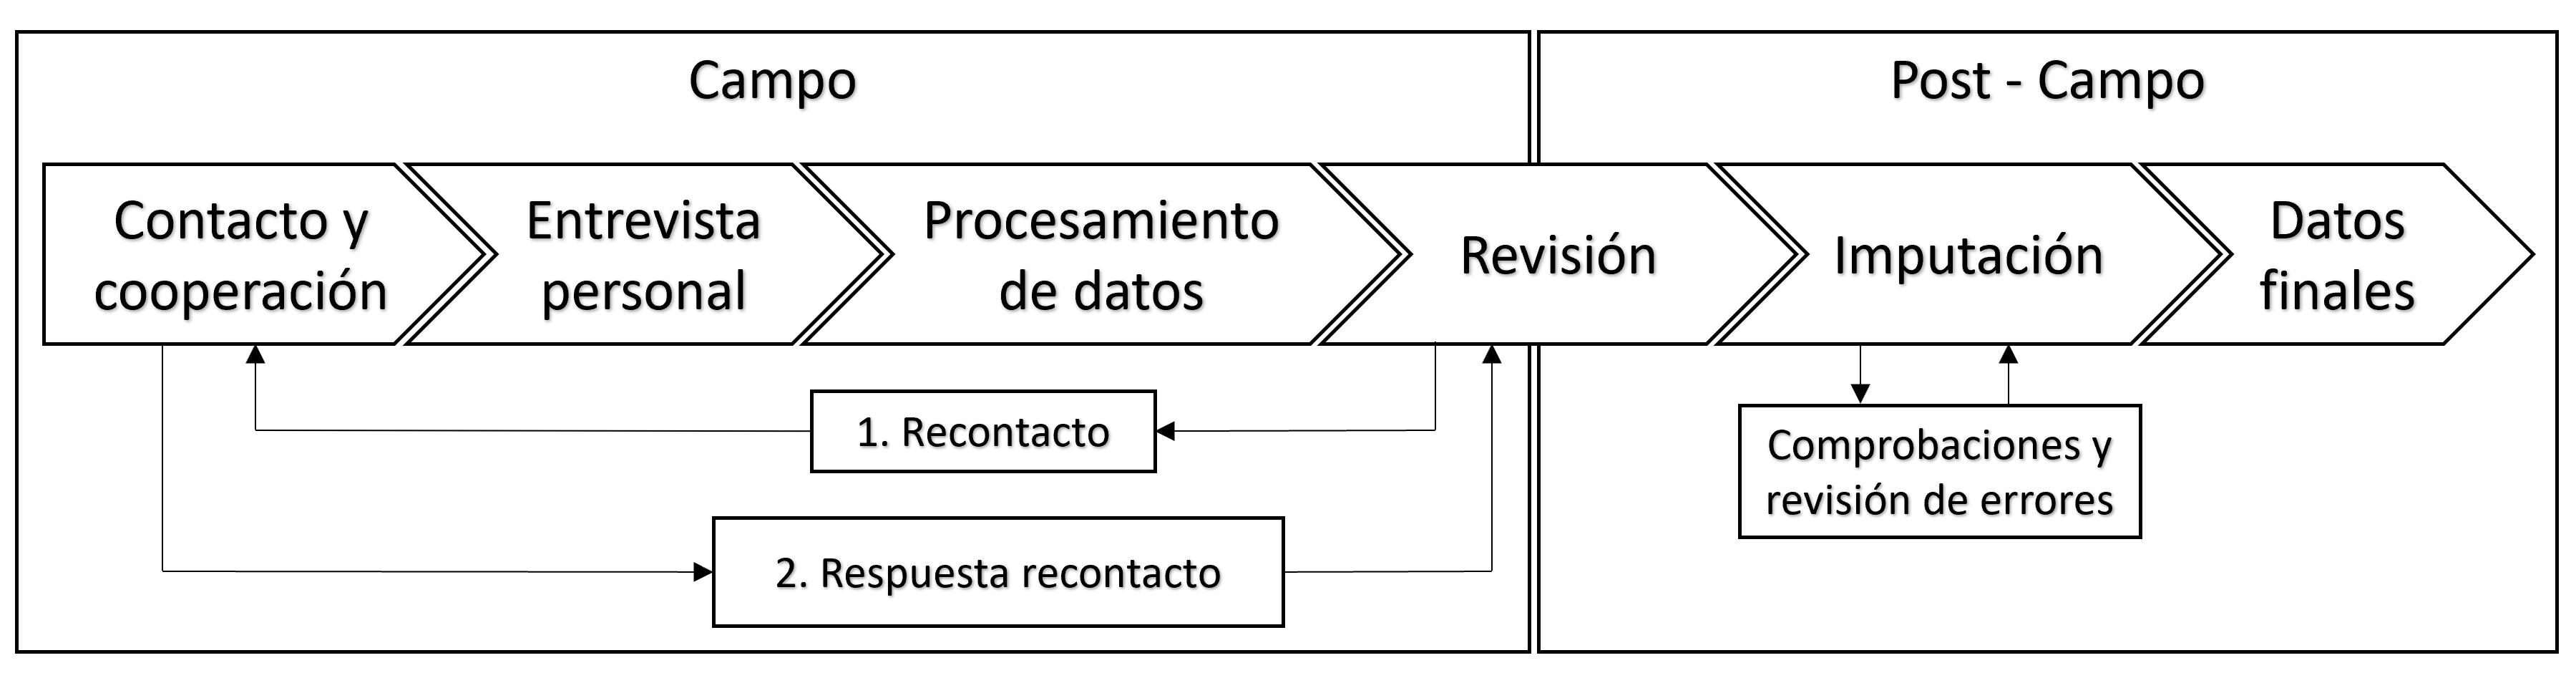
\includegraphics[width=1\textwidth]{figs/fases_creacion_datos_eff.png}
	\caption{Fases de la creación de datos de la EFF}
	\label{fig:eff_phases}
\end{figure}

A continuación se hace una breve descripción de los aspectos más relevantes de las subfases y que son importantes para la selección de variables para este estudio.

\begin{enumerate}[noitemsep]
    \item \textbf{Contacto y cooperación:} Se envía una carta a los hogares para informar sobre su selección para la encuesta y que una persona les visitará personalmente en su domicilio para hacerles una entrevista personal. El contacto puede requerir varias visitas, ya que es necesario que algún miembro del hogar esté físicamente en su hogar cuando tenga lugar la visita presencial. La información sobre cada intento (fecha y hora, resultado...) se recoge en un ordenador. Antes de establecer el contacto, los entrevistadores rellenan un cuestionario que recoge información sobre las características del barrio y del edificio en el que vive el hogar. Los entrevistadores también llevan documentación sobre la encuesta que pueden utilizar para intentar convencer al hogar, como por ejemplo un folleto con noticias de prensa en las que se ha hablado de la EFF.
    \item \textbf{Entrevista personal:} Se realiza una entrevista personal a la persona con más conocimiento de las finanzas del hogar, que se denomina Persona de Referencia o PR. La PR puede ser miembro del hogar, o un representante del mismo, demoninado proxy, siempre y cuando sea la persona con mayor conocimiento de las finanzas del hogar. También pueden participar otros miembros del hogar. Las entrevistas suelen durar entre una hora y hora y media (\cite{effmethod2017}). Antes de empezar la entrevista, se pide a la PR su consentimiento para que algunas partes de la misma puedan ser grabadas en audio por motivos de calidad de los datos. La entrevista puede realizarse aunque no haya grabación. Los entrevistadores recogen las respuestas en un ordenador o una tablet (CAPI), y también pueden anotar en comentarios de texto todos los detalles que consideren importantes para la revisión. La PR puede decidir no contestar a ciertas preguntas. Su valor se asignará como missing, y se imputará más adelante. Las cantidades monetarias pueden responderse en valor puntual, o dentro de un rango de valores. Tras la entrevista, y sin la presencia de los hogares, los entrevistadores rellenan un cuestionario con información sobre el desarrollo de la entrevista, en el que por ejemplo se recoge el nivel de comprensión de la PR a las preguntas, el nivel de interés mostrado por la PR o cuántas personas han participado en la entrevista.
    \item \textbf{Procesamiento de datos:} Los ordenadores y servidores de la empresa de campo procesan los datos recogidos durante el contacto con los hogares y durante las entrevistas. Se crean tres ficheros: uno con las respuestas al cuestionario, otro con la información de los contactos con cada hogar, y finalmente un tercero con la información del paradata recogido por el ordenador durante la entrevista\footnote{También se crea un fichero con los comentarios de texto recogidos por los entrevistadores durante la entrevista, pero no se ha podido incluir en este estudio por falta de tiempo.}.
    \item \textbf{Revisión:} Un equipo de personas revisa individualmente todas las entrevistas y corrige los errores que puedan detectarse. Si hay información relevante que se ha recogido erróneamente o se ha omitido, se contacta de nuevo con el hogar para corregirlo o recuperar esa información. Este recontacto se hace por teléfono. Toda la información sobre la revisión (cambios sobre variables, recontactos...) se recoge en una aplicación informática y puede ser exportada en ficheros de diversos formatos (csv, excel...).
    \item \textbf{Imputación:} Se analiza la proporción de preguntas sin responder dentro de cada entrevista (no-respuesta), y se eliminan las que no superen ciertos umbrales de calidad. Todas las variables que contienen no-respuesta se imputan mediante técnicas de imputación múltiple\footnote{Los métodos de imputación múltiple utilizados en la EFF pueden consultarse en \cite{barcelo2006imputation}.}. Se crean 5 ficheros con datos imputados.
\end{enumerate}

Con respecto a los procedimientos de Contacto y Entrevista personal, es necesario mencionar que algunos elementos tuvieron que modificarse durante la EFF2020, ya que el campo tuvo lugar entre noviembre de 2020 y junio de 2021, y se vió afectado por la pandemia del Covid-19. Durante esa ola, los entrevistadores siguieron visitando personalmente a los hogares para conseguir su colaboración\footnote{Durante el principio del campo, algunos hogares panel fueron contactados sólo por teléfono, pero a las pocas semanas se decidió establecer la visita personal como el procedimiento estándar.}, pero siempre respetando las medidas de distanciamiento social. Las entrevistas se realizaron de manera telefónica asistida por una tablet (CATI). El resto de procedimientos se mantuvieron como en otras ediciones.

\section{Análisis Exploratorio de los Datos}
\label{section:exploring}

Para este proyecto se recopila información de las olas EFF2017, EFF2020 y EFF2022 \footnote{En el momento de escribir este documento, la EFF2022 se encontraba en pleno proceso de imputación, por lo que el equipo del Banco de España ya conocía los resultados de participación de esa ola y era posible utilizarlos para este proyecto.}. Estas ediciones son las únicas que cuentan con la información más detallada de paradata y de las características de los entrevistadores. En ediciones anteriores esta información o no está disponible, o contiene errores de medida que no son fácilmente corregibles. A pesar de esto, es posible identificar en cuántas ediciones ha participado cada hogar, por lo que es posible utilizar información que se remonta hasta la edición de la EFF2011.

En este proyecto se ha manejado una gran cantidad de datos de gran diversidad de origen y formato. El análisis exploratorio de toda esa información es muy amplio y no es posible incluir todo el trabajo realizado en esta sección. Por esa razón, sólo se muestran resultados que son de interés para el análisis del Panel Attrition, o resultados que han ayudado a la toma de decisiones para la selección o transformación de variables para los modelos de predicción.

Este análisis se separa en seis bloques. El primero describe la gran cantidad de datos que se generan en la EFF y el proceso de filtrado de registros y variables que se ha realizado para este proyecto. El segundo bloque trata sobre la existencia de valores perdidos en los datos de la EFF, y cómo se ha solventado. El tercero aborda la existencia de valores atípicos en la EFF, que se limitan a las duraciones de la entrevista. Finalmente, los tres últimos bloques siguientes analizan tres áreas que tradicionalmente se relacionan con el Panel Attrition: la experiencia de los panelistas en la encuesta y las entrevistas, la persona que responde a la encuesta, y las características de los hogares.

\subsection*{Listado de ficheros}
\label{section:files}

En este proyecto se ha combinado información de un total de \textbf{doce ficheros} de datos. Sin embargo, muchos de ellos comparten nombre y contienen el mismo tipo de información, pero hace referencia a olas diferentes de la EFF. Por ejemplo, las respuestas al cuestionario de la EFF se recogen en un fichero llamado "Fichero de trabajo", pero hay uno para la EFF2017 y otro diferente para la EFF2020. En la siguiente lista se especifican los nombres de cada uno de los ficheros utilizados, qué información contienen, y cuántos se utilizan de cada uno en este proyecto.

\begin{itemize}[noitemsep]
    \item \textbf{Fichero de trabajo:} Registros de hogares con entrevistas válidas. Hay uno para cada edición de la encuesta. Contiene la información de las respuestas de los hogares, incluyendo las correcciones y ediciones de la revisión. Se indican los datos que deben ser imputados. También incluye variables auxiliares generadas para el proceso de imputación (características del hogar, de los miembros, del municipio...) y contadores de no respuesta de cada entrevista. Es el fichero que se utiliza para imputar. Se utilizan \textbf{dos ficheros}, el de la EFF2017 y el de la EFF2020.
    \item \textbf{Fichero de datos imputados:} Registros de hogares que contiene las respuestas al cuestionario después de haber imputado los datos con no-respuesta de los hogares. Hay cinco ficheros para cada edición, pero por simplicidad sólo se utiliza uno de los conjuntos de datos de la imputación multiple. Sólo contiene variables imputadas e indicadores de las características del hogar. Aunque durante la imputación múltiple se crean hasta cinco ficheros de datos imputados para cada edición, sólo se utilizará uno de cada edición. En total, se utilizan \textbf{dos ficheros}, los de EFF2017 y EFF2020.
    \item \textbf{Fichero de contactos:} Registos de hogares contactados durante una ola de la EFF. Hay uno para cada ola de la EFF. Contiene información sobre el número de intentos de contacto con cada hogar, la fecha en que se produjo, el resultado de cada uno de ellos (aplazamientos, rechazos...) y las respuestas al cuestionario de vecindario rellenado por los entrevistadores. Se utilizan \textbf{tres ficheros}, los de EFF2017, EFF2020 y EFF2022.
    \item \textbf{Fichero de revisión:} Registros de incidencias durante el proceso de revisión y los recontactos. hay uno para cada edición de la EFF. Contiene información general sobre el proceso de revisión (por ejemplo, si se ha realizado un recontacto), y el resto de registros son incidencias en los datos que se detectado (por ejemplo, si se ha omitido una propiedad inmobiliaria, se abrirá un registro indicando esa incidencia y cómo se ha solucionado). Se utilizan \textbf{dos ficheros}, los de EFF2017 y EFF2020.
    \item \textbf{Fichero de paradata:} Registros de las pantallas visualizadas durante el uso del software CAPI durante cada entrevista. Hay uno para cada edición de la EFF. Cada registro es una pantalla visualizada durante una entrevistacada entrevista y se recoge cómo fue la interacción del entrevistador con el ordenador en esa pantalla durante la entrevista. En concreto, contiene la fecha y hora en la que se cargó la pantalla, si se pasó a la pantalla siguiente (se dió una respuesta), el tiempo que se estuvo visualizando dicha pantalla, si se volvió a la pantalla anterior o incluso si se seleccionó parar la entrevista en esa pantalla. Si en una entrevista se pasó varias veces por una pantalla, esa pantalla tendrá tantos registros como veces se cargó esa pantalla. Es posible agrupar los registros por entrevista, pregunta o sección, y ver el flujo de pantallas que se siguió durante la entrevista. Se utilizan \text{dos ficheros}, los de EFF2017 y EFF2020.
    \item \textbf{Censo de entrevistadores:} Registros de entrevistadores que contiene la información disponible sobre todos los entrevistadores que han participado desde la EFF2014 a la EFF2022. Toda la información está recogida en un \textbf{único fichero} que contiene toda la información, por lo que sólo será necesario usar ése.
\end{itemize}

\subsection*{Número de registros y variables}
\label{section:registers_variables}

El Cuadro \ref{table:registers} muestra el número de registros y variables disponibles en cada uno de los ficheros utilizados en este proyecto. Es importante recalcar que estos números incluyen a todos hogares contactados y a todas variables generadas durante la producción de datos de la EFF en sus ediciones de 2017, 2020 y 2022\footnote{De la EFF2022 sólo se utiliza el fichero de contactos ya que sólo se necesita la información sobre la participación de los hogares panel en dicha edición.}. Tras realizar el filtrado de hogares elegibles para el estudio, se obtiene que los hogares de la EFF2017 elegibles para la EFF2020 son 5,937\footnote{Originalmente se identificaron 5938 hogares de la EFF2017 elegibles para la EFF2020. Pero uno de esos hogares no tenía registros en el fichero de paradata, y se eliminó del conjunto de datos final.} y los hogares elegibles de la EFF2020 para la EFF2022 son 5,505. Con respecto al censo de entrevistadores, sus números incluyen a los 260 entrevistadores que han participado en las ediciones de 2014, 2017, 2020 y 2022. Tras filtrar por las ediciones de 2017 y 2020, se obtiene que en la EFF2017 participaron 69 entrevistadores, mientras que en la EFF2020 participaron 65 entrevistadores, de los cuales 25 personas también participaron en la EFF2017.

\begin{table}[htbp]
\centering
\begin{tabular}{llcc}
\textbf{Nombre del fichero} & \textbf{Unidad registro} & \textbf{Registros} & \textbf{Variables} \\ \hline
Trabajo EFF2017 & Hogares & 6,413 & 6,103 \\
Trabajo EFF2020 & Hogares & 6,313 & 6,497 \\ \hline
Datos imputados EFF2017 & Hogares & 6,413 & 659 \\
Datos imputados EFF2020 & Hogares & 6,313 & 787 \\ \hline
Contactos EFF2017 & Hogares & 14,456 & 640 \\
Contactos EFF2020 & Hogares & 15,457 & 636 \\
Pontactos EFF2020 & Hogares & 15,182 & 636 \\ \hline
Paradata EFF2017 & Pantallas CAPI & 2,807,091 & 13 \\
Paradata EFF2020 & Pantallas CAPI & 3,121,437 & 12 \\ \hline
Revisión EFF2017 & Incidencias & 44,760 & 22 \\
Revisión EFF2020 & Incidencias & 35,217 & 51 \\ \hline
Censo entrevistadores & Entrevistadores & 260 & 56 \\ \hline
\end{tabular}
\caption{\textit{Número de registros y variables de los ficheros de datos}}
\label{table:registers}
\end{table}

En el cuadro \ref{table:registers} también puede observarse que hay ficheros que almacenan más de 6,000 variables. Esto supone un problema de dimensionalidad, ya que hay más variables que registros en los datos. Sin embargo, hay cinco maneras para reducir drásticamente el número de variables a manejar sin perder información relevante, y obtener las variables mencionadas en el cuadro \ref{table:vars}. La primera es que la inmensa mayoría de variables almacenan las respuestas al cuestionario principal de la EFF. En la sección \ref{section:eff} se comenta que el número de preguntas que se formulan depende del número de miembros del hogar, sus edades, y los activos y deudas que posea el hogar, y que en la EFF2017 se plantearon entre 137 y 594 preguntas a cada hogar. Como los modelos de predicción requieren de variables que contengan datos para todos los registros, es posible descartar muchas variables porque no tienen valores para todos los hogares.

La segunda razón para descartar variables es que muchas no son informativas en su estado original y necesitan ser combinadas con otras para poder obtener información interpretable, o se utilizan como apoyo para la imputación. Por ejemplo, la información sobre cantidades monetarias se recoge en cuatro variables que permiten declarar valores en intervalos a los hogares que no quieran o no puedan dar un valor puntual (\cite{effmethod2017}). Esto se utiliza en la imputación para estimar valores puntuales dentro del rango declarado por el hogar. Al usar el fichero de datos imputados para entrenar los modelos, todas esas variables auxiliares se descartan.

En tercer lugar, hay variables duplicadas porque están almacenadas en varios ficheros de datos, por lo que sólo es necesario extraerlas de uno de esos ficheros. Por ejemplo, todas las variables que aparecen en el fichero de datos imputados también aparecen en el fichero de trabajo. Del fichero de trabajo se extraen indicadores de no-respuesta y otras variables de interés que no aparecen en el fichero de datos imputados, y de éste último se extraen las variables con los valores missing imputados.

Finalmente, para que los modelos de predicción puedan entrenarse tanto con datos de la EFF2017 como con la EFF2020, sólo se seleccionan las variables que estaban disponibles en ambas olas. Esta tarea ha requerido una gran dedicación de esfuerzo y tiempo, ya que en algunos ficheros se detectaron variables que no mantuvieron su nomeclatura, el tipo de dato almacenado o la codificación de los datos entre diferentes olas. Para asegurar la homogeneidad, se ha revisado de manera individualizada la nomenclatura y la codificación de cada variable para ambas ediciones de la EFF.

La estructura final de los ficheros es de 5,937 registros de hogares para el conjunto de entrenamiento, y 5,505 registros de hogares para el conjunto de test. Ambos ficheros contienen 57 variables predictoras. Esta información puede consultarse en el cuadro \ref{table:train_test_structure}.

\begin{table}[htbp]
\begin{tabular}{lcccc}
\textbf{Fichero} & \textbf{Unidad de registro} & \textbf{Hogares} & \textbf{Predictores} & \multicolumn{1}{l}{\textbf{Variable a predecir}} \\ \hline
Entrenamiento & Hogares & 5,937 & 57 & Attrition en 2020 \\
Test & Hogares & 5,505 & 57 & Attrition en 2022 \\ \hline
\end{tabular}
\caption{Estructura final de ficheros de entrenamiento y test}
\label{table:train_test_structure}
\end{table}

\subsection*{Valores perdidos en la EFF}
\label{subsection:missing}

En los datos de la EFF hay dos tipos de valores missing: 'verdaderos missing' y 'no-respuesta' de los hogares.

Los 'verdaderos missing' son variables que se corresponden a preguntas del cuestionario que no se plantean al hogar porque las respuestas que han dado anteriormente indican que no deben formularse. Por ejemplo, si un hogar declara que no posee vehículos, no se le formulará la pregunta sobre el valor actual de sus vehículos, por lo que la variable del valor de los vehículos se quedará a missing. Las variables con este tipo de valores perdidos se han descartado del conjunto de datos final, aunque algunas se han utilizado para calcular variables agregadas.

El segundo tipo de valor perdido de la EFF es la 'no-respuesta' de los hogares. Tal y como se ha comentado en la sección \ref{section:etapas_eff}, los hogares pueden decidir no responder a todas las preguntas. Por ejemplo, pueden declarar que tienen cuentas para realizar pagos, pero no decir cuánto es el saldo en esas cuentas. En esos casos se asigna un valor específico que indica que ese dato está missing. Hay muy pocas variables que no contentan al menos una variable con 'no-respuesta'. Eliminarlas reduciría drásticamente el tamaño de la muestra del estudio, e incluso podrían descartarse registros importantes. Por esa razón, la mejor opción es imputar esos valores perdidos. Sin embargo, tal y como se ha mencionado en la sección \ref{section:etapas_eff}, el propio equipo de la EFF ya imputa esos valores durante la producción de los datos finales de la encuesta. Por tanto, se toman esos valores imputados para tratar los valores perdidos debido a la no-respuesta de los hogares.


\subsection*{Valores atípicos en la EFF: duración de las entrevistas}
\label{subsection:outliers}

Para el entrenamiento de modelos de machine learning es importante revisar la existencia de valores atípicos, ya que pueden afectar a sus resultados. Para el tratamiento de estos valores se suele optar por tres opciones: eliminar los registros con valores atípicos, imputar sus valores, o dejarlos porque se consideran valores válidos y cuyos valores pueden ser relevantes para el análisis. En el caso de este proyecto, la opción de eliminar registros se descarta porque los tamaños muestrales ya son bastante reducidos. Por otro lado, durante la producción de la EFF se realizan muchos análisis y revisiones de valores atípicos en los datos, y sólo se dejan sin alterar los que se consideran realmente inverosímiles y no hay sospecha de que pueda haber un error. Por tanto, como ya han pasado varias revisiones, no se van a imputar valores atípicos en variables que provengan de respuestas de los hogares a las preguntas del cuestionario. Esta información incluye variables como la renta o la riqueza.

En cambio, sí se revisan las variables provenientes del paradata o los contactos. En la revisión de la información de contactos no se detecta ningún valor atípico, pero al analizar la distribución de las duraciones de las entrevistas se encontraron entrevistas que duraron más de 20 horas, cuando las entrevistas suelen durar entre una hora y hora y media (\cite{effmethod2017}). La duración total de la entrevista se calcula en segundos, y se obtiene a partir del fichero paradata. Se calcula como la suma de los segundos que pasaron en cada pantalla del CAPI durante la entrevista de cada hogar. Además, como es posible identificar a qué pregunta corresponde cada pantalla, es posible calcular la duración de cada una de las 9 secciones del cuestionario de la EFF. Esta información puede verse en la figura \ref{fig:fig4}.

\begin{figure}[htbp]
	\centering
	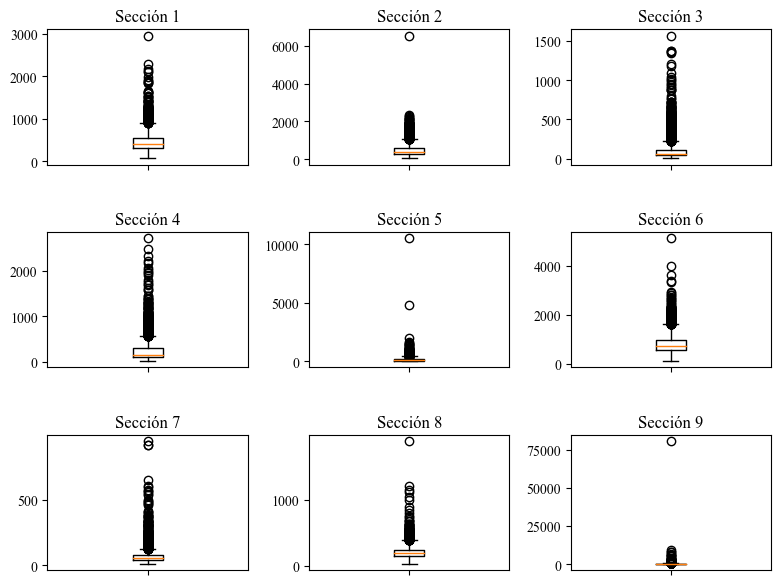
\includegraphics[width=1\textwidth]{figs/figure4.png}
	\caption{Duración por sección del cuestionario en la EFF2017}
	\label{fig:fig4}
\end{figure}

La figura \ref{fig:fig4} contiene los gráficos box-plot de las duraciones de las 9 secciones del cuestionario de la EFF2017. En estos gráficos se ve que hay valores atípicos en todas las secciones, y que algunos son particularmente altos, especialmente en la sección 9. Se sospecha que los entrevistadores no cerraron bien la aplicación del ordenador o la tablet al tomar un descanso, o al interrumpir una entrevista, o al terminarla.

Estos valores tan altos representan un error de medición importante que puede afectar a los modelos de predicción, por lo que es necesario tratarlos. Como hay secciones que contienen más preguntas que otras, la duración en cada sección dependerá de cuántas preguntas se formulen en cada sección. Como el fichero paradata contiene esa información, se decide imputar la duración a nivel de sección, y en concreto se imputan los valores que estén por encima del percentil 99.9 de la duración de dicha sección. Se utiliza el algoritmo kNN (\textit{k-nearest neighbors}) con k=5 y distancia euclídea. Como rasgos de cada sección se calculan el número de preguntas que se formulan una sola vez, el número total de preguntas formuladas, el número de veces que se vuelve a una pantalla anterior, el número de paradas, el número de preguntas categóricas con 1-4 opciones de respuesta, 5-9 opciones de respuesta o más de diez opciones de respuesta, y el tiempo pasado en preguntas monetarias. Tras la imputación, se calcula la duración total de la entrevista como la suma de las duraciones de todas las secciones. Este procedimiento se implementa por separado para las duraciones de cada ola.

\subsection*{Experiencia de hogares en la encuesta y las entrevistas}

En la sección \ref{section:causes_attrition} se comentó que los hogares panel poseen experiencia previa sobre la encuesta que puede afectar a su participación en olas posteriores. Esta experiencia puede abarcar varias ediciones, pero también puede ser informativo observar datos sobre la ola más reciente.

En la figura \ref{fig:fig1} hay cuatro gráficos de mekko que muestran cómo fue la participación en la EFF2020 de hogares elegibles de la EFF2017 según su ola de entrada en la EFF, si consintieron grabar la entrevista de la EFF2017, si dicha entrevista se realizó con un proxy, y el nivel de recelo que mostraron después de realizarla. Los gráficos de mekko son gráficos de columnas apiladas 100\% en los que la anchura de cada columna muestra la proporción de hogares que hay de una categoría dentro de la muestra. Las regiones superiores o rojas de cada columna muestran la proporción de hogares que no participaron en la EFF2020, mientras que las regiones inferiores o azules muestran la proporción de hogares que sí participaron.

\begin{figure}[ht]
	\centering
	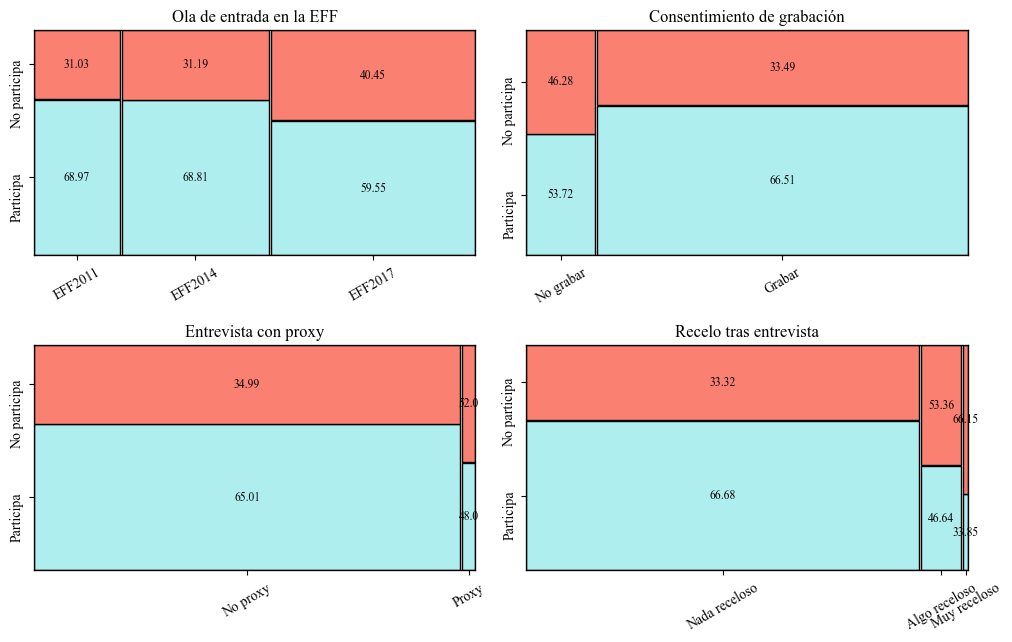
\includegraphics[width=1\textwidth]{figs/figure1.png}
	\caption{Participación en EFF2020 por experiencia en la EFF y en la entrevista de EFF2017}
	\label{fig:fig1}
\end{figure}

En la figura superior izquierda de la figura \ref{fig:fig1} se observa que la proporción de abandono de hogares que participaron por primera vez en 2017 es mayor que la de los que lo hicieron por primera vez en 2014 o en 2011, y entre estas dos últimas la proporción es similar. Esto sugiere que los hogares que van a participar en su segunda ola podrían ser más complicados de retener que los que llevan más tiempo. 

La figura superior derecha muestra que la proporción de no participación es mayor entre los hogares que no consintieron grabar la entrevista en 2017. Esto puede ser una señal de recelo hacia la encuesta, lo que puede dificultar la participación en las siguientes ediciones. En ese sentido también es interesante ver si los hogares se mostraban recelosos tras la entrevista, que es lo que se observa en la figura inferior derecha. La gran mayoría de hogares no se mostraron recelosos tras la entrevista, pero se observa que la proporción de hogares que no participaron en la EFF2020 es mayor a medida que aumenta el nivel de recelo.

Finalmente, en la figura inferior izquierda, se ve que la proporción de abandonos en 2020 fue mayor entre los hogares que hicieron la entrevista con proxy en 2017. Una situación que ha ocurrido bastantes veces en la EFF y que puede encajar con un abandono es el de un hogar formado por personas muy mayores en el que quien lleva las finanzas y termina respondiendo a la entrevista es un hijo o un familiar. Muchos de estos familiares se muestran muy recelosos y, comprensiblemente, quieren que no se moleste a sus familiares. En este tipo de situaciones puede ser más importante volver a convencer a estos familiares que a los propios miembros del hogar, ya que al final son ellos quienes conocen la información del hogar.

Algunos de estos resultados pueden parecer poco útiles porque es razonable pensar que un hogar que se mostró receloso durante la entrevista seguramente será más complicado de convencer para volver a participar en la siguiente edición. Sin embargo, para un entrevistador que está a punto de entrevistar a un hogar, puede ser muy útil saber si ese hogar se mostró receloso tras la anterior entrevista. A la hora convercer al hogar puede centrarse más en utilizar argumentos relacionados con la confidencialidad y la seguridad de los datos y no tanto en hablar de la relevancia de la encuesta o del eco que ha tenido en los medios de comunicación. Estos resultados pueden servir para justificar este tipo de análisis y encontrar qué información puede ayudar al trabajo de los entrevistadores.

\subsection*{Características y comportamiento de la PR}

En la sección \ref{section:causes_attrition} se vió que las características de la persona que responde a una encuesta puede ser relevante para el panel attrition. Es este apartado vamos a ver cómo se relacionan algunas características de la PR en 2017 con la participación del hogar en la EFF2020.

\begin{figure}[ht]
	\centering
	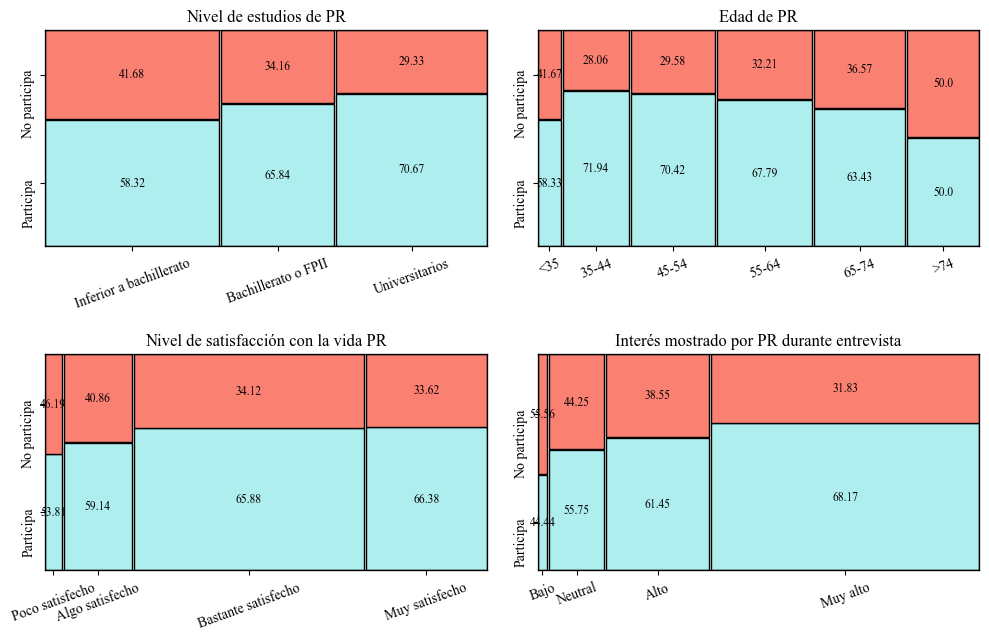
\includegraphics[width=1\textwidth]{figs/figure2.png}
	\caption{Participación en EFF2020 por características y actitudes de PR en EFF2017}
	\label{fig:fig2}
\end{figure}

La figura \ref{fig:fig2} contiene los gráficos de mekko de la participación en la EFF2020 según el nivel máximo de estudios alcanzados de la PR, su edad y su satisfacción con la vida en 2017 y el interés que mostró durante la entrevista de la EFF2017. El gráfico superior izquierdo muestra que la proporción de hogares que no participó en la EFF2020 es mayor cuanto menor era el nivel de estudios de la PR en 2017. Una posible explicación de este resultado podría deberse a la menor tenencia de productos financieros por parte de hogares de menor nivel educativo (\cite{hospido2023encuesta}). El cuestionario de la EFF contiene muchas preguntas sobre muchos productos financieros diferentes, y es razonable pensar que alguien que no posee este tipo de activos piense que no tiene sentido participar en esta encuesta. Un entrevistador con este conocimiento podría preparar un argumentario orientado a destacar que sin su participación no se podría identificar a hogares con sus características y así para poder diseñar políticas económicas específicas para esos hogares.

En el gráfico superior derecho se ve que la proporción de hogares que participó en 2020 aumenta a medida que aumenta la edad de la PR en 2017, excepto cuando ésta tenía menos de 35 años, que presenta la segunda proporción más alta de los grupos de edad. El resultado para los hogares más jóvenes podría explicarse por el hecho de que cada vez menos de estos hogares son propietarios de su vivienda principal (\cite{eff2014results}, \cite{eff2017results}, \cite{eff2020results}) y esto puede hacer que sean más propensos a mudarse, y por tanto ser más difíciles de localizar. El caso de las PR de mayor edad podría explicarse por motivos de fallecimiento.

Finalmente, en los gráficos de la parte inferior de la figura \ref{fig:fig2} vemos, por un lado, que la proporción de hogar que dejan de participar en 2020 se reduce a medida aumenta el nivel de satisfacción con la vida de la PR en 2017, y por otro, que la proporción de hogares que participaron en 2020 aumenta a medida que aumenta el interés por la encuesta. Este último resultado es razonable y útil de saber para el entrevistador porque puede basar su argumentario para convencer al hogar en ese interés.

\subsection*{Características hogar}

En este apartado se analiza a nivel exploratorio la posible relación que puedan tener las características del hogar con el panel attrition. En concreto, se analizan las variables de renta, riqueza y tenencia de deudas. La renta y la riqueza son el eje central de la EFF y es habitual incluirlas de alguna manera en cualquier análisis que se haga con los datos de la encuesta.

En la figura \ref{fig:fig3} hay tres gráficos de mekko en el que se observa la proporción de hogares que participaron en la EFF2020 según la posición relativa de cada hogar en las distribuciones de renta anual y riqueza bruta\footnote{La riqueza bruta se define como la suma del valor de todos los activos que posee el hogar (activos reales + activos financieros = riqueza bruta).} de los hogares españoles en 2017, y también si el hogar tenía deudas pendientes en 2017. La posición relativa de cada hogar dentro de la distribución de renta se muestra indicando los percentiles de la distribución total entre los que se sitúa cada hogar. Si el nivel de renta de un hogar lo sitúa entre los percentiles 60 y 80 del total de la renta de hogares en España, entonces ese hogar está en la categoría "P60-P80" de la distribución de renta, y si se sitúa por encima del percentil 90, la categoría es "\verb|>|P90".

\begin{figure}[ht]
	\centering
	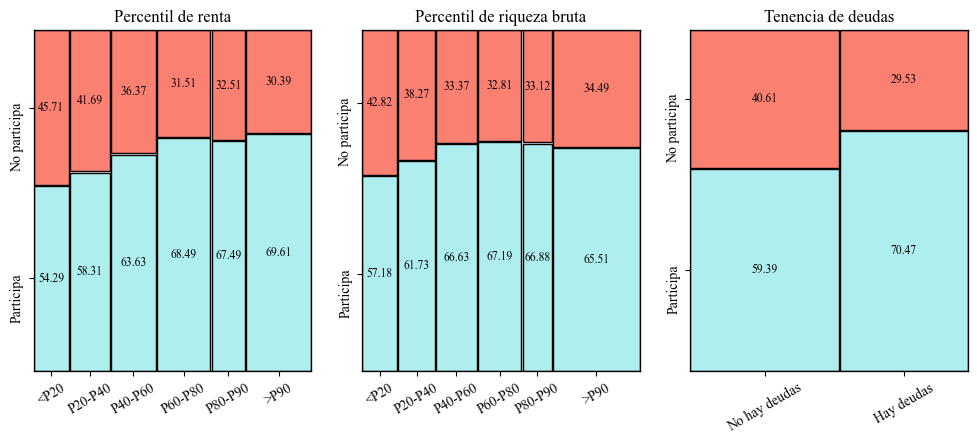
\includegraphics[width=1\textwidth]{figs/figure3.png}
	\caption{Participación en EFF2020 por renta, riqueza y tenencia de deudas en EFF2017}
	\label{fig:fig3}
\end{figure}

En el gráfico de la izquierda de la figura \ref{fig:fig3} se observan dos tendencias diferentes dependiendo del nivel de renta anual de 2017. Por encima del percentil 60 no se aprecian grandes diferencias en la proporción de panelistas que no participaron en 2020, pero por debajo de ese percentil se ve que la proporción de hogares que no participaron es mayor cuanto menor es el nivel de renta. Una posible explicación puede venir de que los niveles de tenencia de activos son menores cuanto menor es el nivel de renta de los hogares (\cite{eff2017results}) y, como se ha comentado para el nivel educativo, es razonable pensar que un hogar que tiene pocos activos considere que no tiene sentido participar en una encuesta como la EFF. Estas dos tendencias también se observan para la distribución de riqueza bruta, pero en este caso la tendencia se observa por debajo del percentil 40 de riqueza bruta. La explicación de por qué la proporción de abandonos es mayor sería similar a la de renta. Si no se tienen activos, se puede pensar que no tiene sentido participar en la EFF.

Finalmente, el gráfico de la derecha muestra la proporción de hogares que participaron en la EFF2020 según si tenían deudas pendientes en 2017. Se observa que la proporción de hogares que no participan en 2020 es mayor entre los hogares que no tenían  deudas en 2017.
\chapter{Resultados}
\label{chapter:resultados}

\section{Evaluación de modelos}
\label{section:evaluation_models}

\subsection*{Rendimiento de los modelos sobre el conjunto de test}

El cuadro \ref{table:test} contiene los resultados de la evaluación de los modelos entrenados con algoritmos de machine learning con respecto al modelo de referencia de Regresión Logística Logit. Recordemos que los modelos se han entrenado con datos de la EFF2017 para predecir la no participación de los hogares panelistas en la EFF2020. El ejercicio del test consistía en predecir la participación de los hogares panel en la ola EFF2022 utilizando información de la EFF2020.

Las métricas de evaluación que se utilizan son Accuracy, Precision, Recall, F1 y ROC AUC. La métrica de referencia que utilizada para la evaluación es la ROC AUC, que se encuentra en la parte derecha del cuadro. Esta métrica mide el rendimiento entre la tasa de falsos positivos y falsos negativos. Toma valores de 0.5 a 1, con 1 siendo un predictor perfecto, y 0.5 el que se obtendría con una estimación realizada de manera aleatoria.

\begin{table}[ht]
    \centering
    \begin{tabular}{lccccc}
    \hline
        \textbf{Modelo} & \textbf{Accuracy} & \textbf{Precision} & \textbf{Recall} & \textbf{F1} & \textbf{ROC AUC} \\ \hline
        Logit & 0,6556 & 0,3749 & 0,3573 & 0,3659 & 0,5959 \\ 
        CART & 0,6434 & 0,3338 & 0,2835 & 0,3066 & 0,5521 \\ 
        Random Forest & 0,6489 & 0,3529 & 0,3148 & 0,3328 & 0,5821 \\ 
        XGBooster & 0,6718 & 0,3772 & 0,2769 & 0,3194 & 0,5911 \\ 
        Naive Bayes & 0,6254 & 0,3504 & 0,4063 & 0,3763 & 0,5798 \\ \hline
    \end{tabular}
    \caption{Métricas de evaluación de los modelos de predicción en el conjunto de test}
    \label{table:test}
\end{table}

El modelo de referencia de este estudio, el Logit, presenta una ROC AUC de 0,5959. La del modelo CART es 0,5521, la del Random Forest es 0,5821, la del XGBooster es 0,5911, y la del Naive Bayes es 0,5798. Ninguno de estos valores mejora a la ROC AUC del modelo Logit. Los que se quedan más cerca son el Random Forest y el XGBooster. De todas maneras, es necesario recalcar que el valor más alto de ROC AUC, el del Logit, sigue estando por debajo de 0,6, por lo que resultados de los test son malos.

\section{¿Por qué el rendimiento de los modelos no es bueno?}

Los resultados de la evaluación de los modelos con el conjunto de test indican que hay modelos de machine learning, aunque se quedan cerca, no mejoran en rendimiento de la predicción con respecto a un Logit. Sin embargo, la métrica ROC AUC por el Logit indica que el rendimiento de este modelo es malo. ¿Por qué los modelos no hacen bien la predicción?

Una posible causa podría ser el overfitting, es decir, que los modelos han aprendido demasiado de los datos con los que han sido entrenados y no son capaces de generalizar bien cuando se enfrentan a datos nuevos. Si esta fuese la principal razón, lo esperable sería que su rendimiento fuese bueno si se hace el ejercicio de predicción sobre los datos de entrenamiento. En el cuadro \ref{table:train} se presenta una comparación entre las métricas de entrenamiento del ejercicio de predecir la Attrition con los datos de test y de entrenamiento (Train).

\begin{table}[ht]
\centering
\begin{tabular}{lcccccc}
\hline
\textbf{Modelo} & \multicolumn{1}{l}{\textbf{Datos}} & \multicolumn{1}{l}{\textbf{Accuracy}} & \multicolumn{1}{l}{\textbf{Precision}} & \multicolumn{1}{l}{\textbf{Recall}} & \multicolumn{1}{l}{\textbf{F1}} & \multicolumn{1}{l}{\textbf{ROC AUC}} \\ \hline
\multirow{2}{*}{Logit} & Test & 0,6556 & 0,3749 & 0,3573 & 0,3659 & 0,5959 \\
 & Train & 0,6389 & 0,4905 & 0,4518 & 0,4704 & 0,6517 \\ \hline
\multirow{2}{*}{CART} & Test & 0,6434 & 0,3338 & 0,2835 & 0,3066 & 0,5521 \\
 & Train & 0,6126 & 0,4594 & 0,5178 & 0,4868 & 0,6188 \\ \hline
\multirow{2}{*}{Random Forest} & Test & 0,6489 & 0,3529 & 0,3148 & 0,3328 & 0,5821 \\
 & Train & 0,6596 & 0,5223 & 0,4770 & 0,4986 & 0,6726 \\ \hline
\multirow{2}{*}{XGBooster} & Test & 0,6718 & 0,3772 & 0,2769 & 0,3194 & 0,5911 \\
 & Train & 0,6544 & 0,5144 & 0,4675 & 0,4898 & 0,6722 \\ \hline
\multirow{2}{*}{Naive Bayes} & Test & 0,6254 & 0,3504 & 0,4063 & 0,3763 & 0,5798 \\
 & Train & 0,6251 & 0,4741 & 0,5178 & 0,4950 & 0,6435 \\ \hline
\end{tabular}
\caption{Comparación métricas evaluación entre conjuntos Test y Train}
\label{table:train}
\end{table}

En esta tabla hay dos tipos de resultados. En primer lugar, se observa que los resultados del test decaen puntos con respecto al conjunto de entrenamiento. Esta degradación es esperable, ya que los algoritmos han sido entrenados con el conjunto de entrenamiento y conocen los patrones internos de los datos mejor que los del conjunto de testo. La caída del entrenamiento al test es baja cuando se compara la métrica de Accuracy, pero la caída es más grande para el resto de métricas. Por ejemplo, la ROC AUC del Random Forest cae de 0,6726 para el conjunto de entrenamiento a 0,5821 para el conjunto de test, y la del Logit cae de 0,6517 para el entremaniento a 0,5959 para el test.

El segundo tipo de resultados se centra en la comparación del rendimiento entre los modelos para el conjunto de entrenamiento. En este caso la ROC AUC de todos los modelos sí supera el valor de 0,6, y también se observa que la de dos de los modelos, el Random Forest y XGBooster, que son 0,6726 y 0,6722 respectivamente, sí son más altas que la ROC AUC del modelo Logit, que es 0,6517. Del resto de métricas, sólo el recall del XGBooster presenta un valor más bajo que el del modelo Logit. De los dos modelos, el mejor sería el Random Forest porque presenta mejores valores en todas las métricas. Sin embargo, aunque este valor sí esté por encima de 0,6, al estar por debajo de 0,75 a este modelo se le clasifica como un predictor regular. Este resultado descarta el overfitting para explicar el mal rendimiento de los modelos, e invita a considerar otras alternativas e incluso nuevos enfoques. Estas opciones se comentan con más detalle en el capítulo \ref{chapter:conclusiones}.

\section{Importancia de las variables para explicar Panel Attrition}

Aunque en los otros dos apartados de este capítulo se ha visto que los modelos de machine learning no han presentado buenos resultados a la hora de predecir el Panel Attrition, puede ser interesante utilizarlos para hacer un ejercicio explicativo en vez de predictivo, e intentar aprender qué información panel puede ser importante para determinar el Attrition. Tal y como se comentó en el capítulo \ref{chapter:metodologia}, una ventaja de los modelos basados en árboles de decisión es que son interpretables, y en concreto los modelos de Random Forest y XGBooster permiten estimar qué variables han tenido más peso a la hora de clasificar la participación de los hogares en la siguiente edición. En este apartado se analizan los resultados del Random Forest, ya que es el que presentó mejores resultados en la predicción utilizando el conjunto de entrenamiento.

El cuadro \ref{table:importance} presenta las 20 variables con más importancia en el modelo de Random Forest ordenadas por valor de importancia.

\begin{table}[ht]
    \centering
    \begin{tabular}{lc}
    \hline
        \textbf{Variable} & \textbf{Importancia} \\ \hline
        PR es panel & 0,0822 \\ 
        Interés PR & 0,0790 \\ 
        Razones para colaborar - Relevancia de la encuesta & 0,0605 \\ 
        Proporción de preguntas monetarias respondidas (incluye intervalos) & 0,0594 \\ 
        Posee al menos un vehículo & 0,0539 \\ 
        Tiene deudas pendientes & 0,0496 \\ 
        Situación laboral - Asalariado & 0,0475 \\ 
        Razones colaborar - Interesado en estos estudios & 0,0380 \\ 
        Posee planes de pensiones & 0,0353 \\ 
        PR consiente grabar la entrevista & 0,0348 \\ 
        Hijos viven en el hogar & 0,0318 \\ 
        Nivel educativo PR & 0,0313 \\ 
        Número de olas en las que ha participado el hogar & 0,0304 \\ 
        Sexo de PR & 0,0291 \\ 
        Número de adultos con trabajo & 0,0277 \\ 
        Posee fondos de inversión & 0,0206 \\ 
        Nivel de comprensión de las preguntas por PR & 0,0206 \\ 
        Proporción de preguntas monetarias respondidas en valor puntual & 0,0198 \\ 
        Razones para colaborar - El estudio lo lleva el BdE & 0,0195 \\ 
        Estado Civil - Casada & 0,0190 \\ \hline
    \end{tabular}
    \caption{Importancia de las variables en el modelo de Random Forest}
    \label{table:importance}
\end{table}

La importancia de una variable en el Random Forest mide el peso relativo que ha tenido una variable concreta a la hora de crear las ramificaciones de los diferentes árboles de decisiones que va generando el Random Forest durante su entrenamiento. En la participación en la EFF2020, las tres variables que más importancia tuvieron fueron que la PR fuera panel, que la PR mostrase interés durante la entrevista, y que el entrevistador indicase que el hogar colaboró por la relevancia de la encuesta. También es interesante destacar la importancia de proporción de preguntas monetarias respondidas por el hogar (incluyendo intervalos), y algunas variables que hemos mencionado en la sección \ref{section:exploring}, como son si la PR consintió que se grabase la entrevista, el nivel educativo de la PR y el número de olas en las que el hogar ha participado.
\chapter{Conclusiones y líneas de trabajo futuras}
\label{chapter:conclusiones}

El objetivo principal de este Trabajo de Fin de Máster es desarrollar un modelo basado en algoritmos de machine learning que ayude a predecir si un hogar panel de la Encuesta Financiera de las Familias (EFF) dejará de participar en la siguiente edición. Para ello, se ha seguido la implementación de entrenamiento y evaluación realizada en \cite{beste2023case}, pero adaptada al caso de estudio de la EFF.

Este trabajo se ha divido en dos piezas de análisis. La primera es un análisis exploratorio de las variables de la EFF y ver su posible relación con la participación de los hogares en la siguiente edición. En la segunda se entrenan cuatro modelos basados en algoritmos de machine learning (CART, Random Forest, XGBooster y Naïve-Bayes) para predecir el Panel Attrition en la EFF2020 con datos de la EFF2017, y a continuación se compara y evalúa su rendimiento comparado con el ofrecido por un modelo de Regresión Logística de efectos principales, que es un modelo que se ha utilizado tradicionalmente para analizar el Panel Attrition.

El trabajo de análisis exploratorio ha supuesto un desafío ya que ha requerido manejar, combinar y homogeneizar información de un total de doce ficheros de datos repartidos entre tres ediciones de la EFF. Siete de ellos contenían registros de hogares, otros dos registros de incidencias, otros dos registros de pantallas de interacción con un software y el último era un censo de entrevistadores. Además, dos de los ficheros contenían más de 6,000 variables, y otros dos más de 600. En una misma edición de la encuesta había algunas variables duplicadas en diferentes ficheros, y también algunas variables comunes entre olas tenían diferentes codificaciones dependiendo de la ola. Tras eliminar duplicados, redundancias y homogeneizar variables, se consiguió un conjunto de datos para el entrenamiento de 5,397 hogares y 57 variables predictoras.

El análisis exploratorio ha mostrado varios resultados interesantes que pueden ser útiles para hacer implementaciones de diseños adaptativos. La proporción de hogares panel que no participaron en la EFF2020 era mayor para hogares que en 2017 participaron por primera vez, se mostraron más recelosos, no consintieron grabar la entrevista, la realizaron con un proxy. También lo era en aquellos hogares cuya PR en 2017 tenía un menor nivel de estudios, tenía menos de 35 años o más de 74, mostraron un menor nivel de satisfacción con su vida y un menor interés durante la entrevista. Finalmente, la proporción de abandonos en 2020 también fue mayor para los hogares cuya renta de 2017 se situaba en las tres quintilas inferiores de la distribución de renta de los hogares españoles en 2017, su riqueza bruta en 2017 se encontrada en dos las quintilas inferiores de la distribución de riqueza bruta de todos los hogares españoles en 2017, y si no poseían deudas. Toda esta información puede ser útil para un entrevistador que va a visitar a un hogar panel porque puede adaptar los argumentos que utilice para convencerles. Por ejemplo, si el hogar se mostró receloso en la edición anterior, puede ser más útil enfocarse en hablar sobre la confidencialidad de la encuesta que la presencia del estudio en los medios de comunicación.

En la parte del entrenamiento y evaluación de los modelos de machine learning, ninguno de los modelos de machine learning entrenados llega a superar el rendimiento del modelo de Regresión Logística para la predicción del conjunto de test. Además, el valor de la ROC AUC de este modelo Logit no supera el valor de 0.6, lo cual lo clasifica como un predictor malo. Para intentar aprender sobre los errores de predicción, se han usado esos mismos modelos para hacer la predicción con el conjunto de entrenamiento y hacer una comparación entre los resultados del conjunto de test y los de entrenamiento. Todos los modelos presentan mejores resultados para el conjunto que entrenamiento que para el de test, y además los modelos de Random Forest y XGBooster sí presentan valores más altos de ROC AUC que el modelo Logit. Sin embargo, la mejor métrica, la del Random Forest, no llega a superar el valor de 0,7, que lo clasifica como un predictor regular. No parece que los modelos hagan overfitting.

Finalmente, para aprender cómo ha sido el entrenamiento del Random Forest, se observa la importancia de los veinte predictores con mayor valor de importancia. Destacan que la PR ya formase parte del hogar desde al menos dos ediciones antes, el valor del interés mostrado por la PR, que el entrevistador considerase que el hogar participó por la relevancia de la encuesta y algunas variables analizadas durante la exploración de los datos, en concreto la tenencia de deudas pendientes, el número de olas en las que ha participado el hogar, que la PR consintiera grabar la entrevista y el nivel educativo de la PR.

A partir de los resultados que se han visto en este proyecto, se plantean las siguientes reflexiones y los posibles pasos que se podrían dar en el futuro para este proyecto:

\begin{enumerate}
    \item \textbf{Revisar la selección de variables:} Un buen modelo predictivo requiere estar construido sobre variables que tengan poder predictivo sobre la variable de interés. Los resultados del análisis descriptivo muestran que las variables seleccionadas tienen relación con la participación de los hogares, pero no tienen suficiente poder para predecir la participación de los hogares en las ediciones siguientes. La selección de variables se inspiró en las implementaciones de \cite{kern2021predicting} y \cite{beste2023case}, que son ejemplos de buenas predicciones de Panel Attrition de hogares. Pero aunque sean encuestas a hogares, tienen métodos de recolección de datos, frecuencias y muestreos diferentes al de la EFF, y en \cite{jankowsky2022validation} mencionan que esos factores pueden afectar a los resultados de los modelos e impedir su generalización a otras encuestas. Afortunadamente, en la EFF se recogen muchas variables que no se han utilizado en este estudio, y su inclusión podría mejorar el rendimiento de los modelos hasta niveles aceptables. Esto abre vías de trabajo futuro continuistas:
    \begin{enumerate}[noitemsep]
        \item Revisar la selección de variables actual, añadir las que se hayan dejado fuera y puedan tener poder predictivo, y eliminar aquellas que puedan estar generando ruido. Implementar procesos de feature selection basados en algoritmos de machine learning.
        \item Hacer un análisis más profundo del error de predicción. En concreto, analizar de manera específica aquellos hogares que los modelos predicen mal y ver qué características tienen.
    \end{enumerate}
    \item \textbf{Plantear un ejercicio explicativo en vez de predictivo:} Todo ejercicio de predicción requiere utilizar variables que se conozcan ex-ante. Por esa razón, los modelos de predicción de Panel Attrition utilizan los datos de ediciones anteriores como predictores. Pero la predicción sólo saldrá bien si esos datos tienen mayor influencia sobre el resultado de la variable objetivo que otras variables que todavía se desconocen. Por ejemplo, el papel del entrevistador es muy importante para conseguir la colaboración de los hogares y para conseguir datos de calidad (\cite{lynn2018tackling} y \cite{groves2006nonresponse}). Pero es imposible saber qué entrevistadores estarán disponibles para el trabajo de campo hasta que llegue el momento de hacer las entrevistas. En este sentido, antes de continuar con el ejercicio predictivo, puede ser interesante utilizar todos los datos disponibles de todas las olas y hacer un análisis explicativo de los factores que determinan la participación de los hogares panel, diferenciando entre variables conocidas ex-ante y variables ex-post, y comprobando cuál de los dos grupos tienen más influencia.
    \item \textbf{El posible papel del Covid-19:} Las olas de la EFF seleccionadas para el estudio son EFF2017, EFF2020 y EFF2022 porque son las que tienen mayor cantidad de datos y también los de mayor calidad. Sin embargo, como se comentó en la sección \ref{chapter:datos}, la pandemia del Covid-19 obligó a cambiar la metodología del campo de la EFF2020 para poder hacer la encuesta respetando las condiciones de seguridad y distancia social. Todos los modelos entrenados utilizan datos de 2017 para predecir 2020, que es año de Covid. Y posteriormente, en el test se utiliza información recogida durante 2020, de nuevo Covid, para predecir 2022, cuando ya se estaba superando la pandemia y fue posible las entrevistas presenciales. Es muy razonable pensar que muchos hogares rechazaron participar en 2020 por miedo al Covid, y también pensar que cambiar el modo de entrevista de personal a telefónica pudo afectar a los datos. Esto puede implicar que las causas de participación en 2020 sean muy diferentes a las de 2022. Ante esta problemática, se plantean dos posibles alternativas:
    \begin{enumerate}[noitemsep]
        \item \textbf{Hacer un modelo de predicción con los datos de las olas previas a 2020:} La metodología de todas estas olas es homogénea porque todas las entrevistas fueron personales, y no hubo una crisis como la del Covid-19. El inconveniente es que sólo se podría utilizar la información de las respuestas de los hogares. Pero no está claro si necesariamente el rendimiento sería peor.
        \item \textbf{Repetir el actual ejercicio cuando haya más ediciones posteriores a 2020:} La EFF va a continuar realizándose en los próximos años con una frecuencia bienal. Se puede volver a plantear esta misma metodología dentro unos años utilizando sólo ediciones completadas después de 2020, y con el beneficio de recoger toda la información que se recoge actualmente y que no está disponible para antes de 2017.
    \end{enumerate}
    \item\textbf{Cambiar el enfoque:}: Siempre existe la opción de considerar enfoques alternativos sean interesantes y más adecuados para el problema que se quiere abordar. En ese sentido, hay dos alternativas bastante interesantes:
    \begin{enumerate}[noitemsep]
        \item \textbf{Predecir la participación de los paneles en su segunda ola}: En la exploración de los datos se vio que los hogares que han participado sólo en una edición muestran más proporción de abandonos que los que han participado más de dos años. Esto invita a pensar que los hogares que han participado más de una vez están más comprometidos con el estudio, y seguramente merezca la pena enfocar el análisis en la predicción de la participación de los panelistas que sólo han participado una vez en lugar de predecir la participación de todos los hogares.
        \item \textbf{Realizar un análisis de supervivencia:} En vez de predecir un resultado binario, de participar o no participar, se puede plantear hacer un ejercicio de análisis de supervivencia (survival analysis), e intentar predecir el número de ediciones en las que participará un hogar de la EFF antes de abandonar el estudio.
    \end{enumerate}
\end{enumerate}


% bibliografia
\addcontentsline{toc}{chapter}{Bibliografía}
\bibliographystyle{apalike}
\bibliography{referencias}

\end{document}